\lstset{style=mylststyle}
\begin{sloppypar}


\chapter{Detalii de implementare ale problemei}
În acest capitol voi detalia implementarea algoritmului, dar și modul în care Dafny evaluează corectitudinea și optimalitatea codului. 

\section{Reprezentarea datelor de intrare/ieșire}

Pentru a reprezenta problema pentru care algoritmul trebuie să obțină cel mai bun profit pe setul de intrare, am ales sa definesc un tip de date \formatText{Problem} astfel:

\begin{Verbatim}[commandchars=\\\{\}]
\PY{k+kd}{datatype} \PY{n+nc}{Problem} \PY{o}{=} \PY{n}{Problem}\PY{p}{(}\PY{n}{n}\PY{p}{:} \PY{k+kt}{int}\PY{p}{,} \PY{n}{c}\PY{p}{:} \PY{k+kt}{int}\PY{p}{,} \PY{n}{gains}\PY{p}{:} \PY{k+kt}{seq}\PY{o}{\PYZlt{}}\PY{k+kt}{int}\PY{o}{\PYZgt{}}\PY{p}{,} 
\PY{n}{weights}\PY{p}{:} \PY{k+kt}{seq}\PY{o}{\PYZlt{}}\PY{k+kt}{int}\PY{o}{\PYZgt{}}\PY{p}{)} 
\end{Verbatim}
unde:
\begin{itemize}
    \item câmpul \textit{\textbf{\textcolor{coleight}{n}}} reprezintă numărul de obiecte disponibile;
    \item câmpul \textit{\textbf{\textcolor{coleight}{c}}} reprezintă capacitatea totală a rucsacului;
    \item câmpul \textit{\textbf{\textcolor{coleight}{gains}}} este o secvență ce memorează profitul fiecărui obiect;
    \item câmpul \textit{\textbf{\textcolor{coleight}{weights}}} este o secvență ce memorează greutatea fiecărui obiect.
\end{itemize} \par
Folosind cuvântul cheie \formatText{datatype} am definit un nou tip de date inductiv numit \formatText{Problem} cu un singur constructor având același nume în care câmpurile sunt separate prin virgulă și sunt tipuri de date primitive.
\par
Atât profitul, cât și greutatea fiecărui obiect pot fi accesate prin indexul corespunzător poziției din secvență. Spre exemplu, pentru a accesa greutatea celui de-al doilea obiect este folosit operatorul de indexare $weights[1]$, deoarece indexarea celor două secvențe începe de la 0. În dafny, o \textit{secvență} este o colecție de elemente de același tip, iar în cazul acesta, de numere întregi. \\ \par

Datele de ieșire sunt reprezentate astfel:
\begin{Verbatim}[commandchars=\\\{\}]
                \PY{p}{(}\PY{n}{profit}\PY{p}{:} \PY{k+kt}{int}\PY{p}{,} \PY{n}{solution}\PY{p}{:} \PY{n}{Solution}\PY{p}{)}
\end{Verbatim}
unde:
\begin{itemize}
    \item \formatText{profit} reprezintă profitul maxim care se poate obține pentru o anumită instanță a problemei;
    \item \formatText{solution} reprezintă un sinonim al tipului de date \texttt{seq\(<\)int\(>\)} folosit pentru a îmbunătăți claritatea codului, este declarat anterior astfel:
\begin{Verbatim}[commandchars=\\\{\}]
                \PY{n}{type} \PY{n}{Solution} \PY{o}{=} \PY{k+kt}{seq}\PY{o}{\PYZlt{}}\PY{k+kt}{int}\PY{o}{\PYZgt{}}
\end{Verbatim}
și este o reprezentare binară a deciziei de includere a obiectului în rucsac. Prin urmare, valoarea de 1 reprezintă faptul că obiectul aparține soluției, deci este adăugat în rucsac, iar profitul adus de acesta îmbunătățește câștigul final, iar 0 reprezintă faptul că obiectul nu este adăugat în rucsac, deci profitul obiectului nu este inclus în câștigul maxim obținut. Această secvență reprezintă soluția finală care trebuie să fie optimă pentru problema completă.
\end{itemize} 

\section{Soluția optimă și soluțiile parțiale optime}

În cadrul problemei rucsacului putem discuta despre ce reprezintă soluția optimă, cât și soluțiile parțiale optime. \par
Pentru a stoca rezultatele corespunzătoare câștigurilor subproblemelor am folosit o matrice numită \texttt{profits} de tip \texttt{seq<seq<int>>}, iar rezultatele pot fi accesate folosind operatorul de indexare pentru un tablou bidimensional: $profits[i][j]$, unde $i$ și $j$ reprezită mărimea subproblemei pe care încercăm să o rezolvăm.
\par
Pe lângă matricea \texttt{profits}, această lucrare se mai bazează și pe o matrice suplimentară numită \texttt{solutions} de tip \texttt{seq<seq<seq<int>>>} care va stoca fiecare secvență binară corespunzătoare profitului stocat în matricea \texttt{profits}. Rezultatele sunt accesate similar matricei profits.
\par
O \formatText{soluție optimă} reprezintă selecția de obiecte care maximizează profitul format din câștigul fiecărui item care poate fi adăugat în rucsac, dar care în același timp respectă constrângerile legate de capacitatea rucsacului pentru problema completă. Acest rezultat trebuie să fie cel mai bun pe care îl putem obține pentru instanța problemei pe care o primim la intrare, iar această soluție este găsită în ultima celulă a matricei, $solutions[n][c]$.
\par
O \formatText{soluție parțială} este o secvență binară de o lungime variabilă (care nu depășește numărul de obiecte) care respectă constrângerea legată de capacitatea rucsacului. \par
O \formatText{soluție optimă parțială} reprezintă un rezultat optim intermediar calculat pentru un subset de obiecte sau pentru o capacitate parțială a rucsacului. Luând exemplul prezentat în introducere, o soluție parțială pentru subproblema $(i = 3, j = 8)$ este $[0, 1, 1]$ și aduce cel mai bun profit pentru un subset ce include doar primele trei obiecte, având la dispoziție un rucsac de capacitate maximă 8.

\section{Precondiții, postcondiții și invarianți}

\formatText{Precondițiile}, \formatText{postcondițiile} și \formatText{invarianții} mai sunt numite și specificații și reprezintă proprietăți logice folosite pentru a descrie comportamentul pe care ar trebui să îl îndeplinească programul într-un anumit punct al algoritmului. Ele garantează că aceste proprietăți sunt respectate pe tot parcursul execuției și pot fi folosite pentru metode, funcții, bucle, leme și iteratori. \par
Specificațiile sunt esențiale pentru ajutarea verificatorului, permițând astfel validarea corectitudinii logice a programului. Vom considera mai departe această bucată de cod ce aparține unei leme folosite pentru demonstrarea faptului că o soluție este parțială prin adăugarea unui obiect:
\begin{Verbatim}[commandchars=\\\{\}]
\PY{k+kd}{lemma} \PY{n+nf}{computeWeightFits1}\PY{p}{(}\PY{n}{p}\PY{p}{:} \PY{n}{Problem}\PY{p}{,} \PY{n}{solution}\PY{p}{:} \PY{n}{Solution}\PY{p}{,} 
    \PY{n}{i}\PY{p}{:} \PY{k+kt}{int}\PY{p}{,} \PY{n}{j}\PY{p}{:} \PY{k+kt}{int}\PY{p}{)}
  \PY{k}{requires} \PY{n}{isValidProblem}\PY{p}{(}\PY{n}{p}\PY{p}{)}
  \PY{k}{requires} \PY{l+m+mi}{0} \PY{o}{\PYZlt{}=} \PY{o}{|}\PY{n}{solution}\PY{o}{|} \PY{o}{\PYZlt{}} \PY{n}{p}\PY{p}{.}\PY{n}{n}
  \PY{k}{requires} \PY{n}{hasAllowedValues}\PY{p}{(}\PY{n}{solution}\PY{p}{)}
  \PY{k}{requires} \PY{l+m+mi}{0} \PY{o}{\PYZlt{}=} \PY{n}{j} \PY{o}{\PYZlt{}=} \PY{n}{p}\PY{p}{.}\PY{n}{c} \PY{o}{+} \PY{l+m+mi}{1}
  \PY{k}{requires} \PY{n}{i} \PY{o}{==} \PY{o}{|}\PY{n}{solution}\PY{o}{|}
  \PY{k}{requires} \PY{n}{weight}\PY{p}{(}\PY{n}{p}\PY{p}{,} \PY{n}{solution}\PY{p}{)} \PY{o}{\PYZlt{}=} \PY{n}{j} \PY{o}{\PYZhy{}} \PY{n}{p}\PY{p}{.}\PY{n}{weights}\PY{p}{[}\PY{n}{i}\PY{p}{]}
  
  \PY{k}{ensures} \PY{n}{computeWeight}\PY{p}{(}\PY{n}{p}\PY{p}{,} \PY{n}{solution} \PY{o}{+} \PY{p}{[}\PY{l+m+mi}{1}\PY{p}{]}\PY{p}{,} \PY{o}{|}\PY{n}{solution} \PY{o}{+} \PY{p}{[}\PY{l+m+mi}{1}\PY{p}{]}\PY{o}{|} \PY{o}{\PYZhy{}} \PY{l+m+mi}{1}\PY{p}{)} \PY{o}{\PYZlt{}=} \PY{n}{j}
\PY{p}{\PYZob{}}
  \PY{k+kd}{var} \PY{n}{s} \PY{o}{:=} \PY{n}{solution} \PY{o}{+} \PY{p}{[}\PY{l+m+mi}{1}\PY{p}{]}\PY{p}{;}
  \PY{k}{assert} \PY{n}{solution} \PY{o}{==} \PY{n}{s}\PY{p}{[}\PY{p}{..}\PY{o}{|}\PY{n}{s}\PY{o}{|} \PY{o}{\PYZhy{}} \PY{l+m+mi}{1}\PY{p}{]}\PY{p}{;}

  \PY{n}{for} \PY{n}{a} \PY{o}{:=} \PY{l+m+mi}{0} \PY{n}{to} \PY{o}{|}\PY{n}{s}\PY{p}{[}\PY{p}{..}\PY{o}{|}\PY{n}{s}\PY{o}{|} \PY{o}{\PYZhy{}} \PY{l+m+mi}{1}\PY{p}{]}\PY{o}{|}
    \PY{k}{invariant} \PY{l+m+mi}{0} \PY{o}{\PYZlt{}=} \PY{n}{a} \PY{o}{\PYZlt{}=} \PY{o}{|}\PY{n}{s}\PY{p}{[}\PY{p}{..}\PY{o}{|}\PY{n}{s}\PY{o}{|} \PY{o}{\PYZhy{}} \PY{l+m+mi}{1}\PY{p}{]}\PY{o}{|} \PY{o}{+} \PY{l+m+mi}{1}
    \PY{k}{invariant} \PY{k}{forall} \PY{n}{k} \PY{p}{::} \PY{l+m+mi}{0} \PY{o}{\PYZlt{}=} \PY{n}{k} \PY{o}{\PYZlt{}} \PY{n}{a} \PY{o}{==}\PY{o}{\PYZgt{}} 
        \PY{n}{computeWeight}\PY{p}{(}\PY{n}{p}\PY{p}{,} \PY{n}{solution}\PY{p}{,} \PY{n}{k}\PY{p}{)} \PY{o}{==} \PY{n}{computeWeight}\PY{p}{(}\PY{n}{p}\PY{p}{,} \PY{n}{s}\PY{p}{,} \PY{n}{k}\PY{p}{)}
  \PY{p}{\PYZob{}} \PY{p}{\PYZcb{}}
\PY{p}{\PYZcb{}}
\end{Verbatim}
Astfel avem:
\begin{itemize}
    \item \formatText{Precondițiile} sunt expresii logice care trebuie să fie adevărate înainte de executarea logicii unei functii sau metode și necesită clauza \texttt{requires}:
    \begin{Verbatim}[commandchars=\\\{\}]
  \PY{k}{requires} \PY{n}{isValidProblem}\PY{p}{(}\PY{n}{p}\PY{p}{)}
\end{Verbatim}
Această precondiție, spre exemplu, ne asigură că vom lucra în cadrul lemei cu o problemă validă.
\item \formatText{Postcondițiile} sunt expresii logice care trebuie să fie adevărate după executarea logicii unei funcții sau metode și necesită clauza \texttt{ensures}:
    \begin{Verbatim}[commandchars=\\\{\}]
  \PY{k}{ensures} \PY{n}{computeWeight}\PY{p}{(}\PY{n}{p}\PY{p}{,} \PY{n}{solution} \PY{o}{+} \PY{p}{[}\PY{l+m+mi}{1}\PY{p}{]}\PY{p}{,} \PY{o}{|}
    \PY{n}{solution} \PY{o}{+} \PY{p}{[}\PY{l+m+mi}{1}\PY{p}{]}\PY{o}{|} \PY{o}{\PYZhy{}} \PY{l+m+mi}{1}\PY{p}{)} \PY{o}{\PYZlt{}=} \PY{n}{j}
\end{Verbatim}
    Singura postcondiție ne asigură faptul că la ieșirea din lemă putem garanta că pentru parametrii de intrare care respectă precondițiile, expresia logică din postcondiție este adevarată.
    \item \formatText{Invarianții} sunt expresii logice care de obieci sunt folosiți pentru specificațiile unei bucle și trebuie să fie adevărate pe toată durata ciclului, inclusiv înainte de intrarea în buclă, cât și după ieșirea din aceasta. Pentru invarianți se folosește clauza \texttt{invariant}:
    \begin{Verbatim}[commandchars=\\\{\}]
\PY{k}{invariant} \PY{l+m+mi}{0} \PY{o}{\PYZlt{}=} \PY{n}{a} \PY{o}{\PYZlt{}=} \PY{o}{|}\PY{n}{s}\PY{p}{[}\PY{p}{..}\PY{o}{|}\PY{n}{s}\PY{o}{|} \PY{o}{\PYZhy{}} \PY{l+m+mi}{1}\PY{p}{]}\PY{o}{|} \PY{o}{+} \PY{l+m+mi}{1}
\end{Verbatim}
    Invariantul acesta verifică respectarea limitelor valorilor luate de \texttt{a} în cadrul buclei \texttt{for}. Acest invariant este verificat înainte de începerea executării buclei \texttt{for}, cât și pe parcursul fiecărei iterații și după ieșirea din buclă.
\end{itemize}

\section{Predicate și Funcții}

\subsection{Predicate}

Predicatele în Dafny sunt funcții ale călor rezultate sunt valori boolene. Acestea sunt folosite pentru a evalua proprietăți care de obicei trebuie să fie adevărate și de aceea ele ajută în procesul de verificare al corectitudinii. Predicatele pe care urmează să le prezint au fost foarte des folosite ca și condiții pe care metodele și lemele trebuie să le respecte, dar și ca rezultate la ieșirea din acestea pentru asigurarea unor proprietăți necesare, de exemplu, în verificarea optimalității. \par
Astfel, voi continua cu prezentarea predicatelor folosite de mine:
\begin{enumerate}
    \item Predicatul \formatText{hasPositiveValues} este definit astfel:
    \begin{Verbatim}[commandchars=\\\{\}]
\PY{k+kd}{predicate} \PY{n+nf}{hasPositiveValues}\PY{p}{(}\PY{n}{arr}\PY{p}{:} \PY{k+kt}{seq}\PY{o}{\PYZlt{}}\PY{k+kt}{int}\PY{o}{\PYZgt{}}\PY{p}{)}
\PY{p}{\PYZob{}}
  \PY{k}{forall} \PY{n}{i} \PY{p}{::} \PY{l+m+mi}{0} \PY{o}{\PYZlt{}=} \PY{n}{i} \PY{o}{\PYZlt{}} \PY{o}{|}\PY{n}{arr}\PY{o}{|} \PY{o}{==}\PY{o}{\PYZgt{}} \PY{n}{arr}\PY{p}{[}\PY{n}{i}\PY{p}{]} \PY{o}{\PYZgt{}} \PY{l+m+mi}{0}
\PY{p}{\PYZcb{}}
\end{Verbatim}
    și este folosit, după cum sugerează și numele acestuia, pentru a verifica dacă toate elementele unui vector precum $gains$ sunt pozitive.
    \item Predicatul \formatText{hasAllowedValues}
    \begin{Verbatim}[commandchars=\\\{\}]
\PY{k+kd}{predicate} \PY{n+nf}{hasAllowedValues}\PY{p}{(}\PY{n}{solution}\PY{p}{:} \PY{n}{Solution}\PY{p}{)}
\PY{p}{\PYZob{}}
  \PY{k}{forall} \PY{n}{k} \PY{p}{::} \PY{l+m+mi}{0} \PY{o}{\PYZlt{}=} \PY{n}{k} \PY{o}{\PYZlt{}} \PY{o}{|}\PY{n}{solution}\PY{o}{|} \PY{o}{==}\PY{o}{\PYZgt{}} \PY{n}{solution}\PY{p}{[}\PY{n}{k}\PY{p}{]} \PY{o}{==} \PY{l+m+mi}{0} 
        \PY{o}{|}\PY{o}{|} \PY{n}{solution}\PY{p}{[}\PY{n}{k}\PY{p}{]} \PY{o}{==} \PY{l+m+mi}{1}
\PY{p}{\PYZcb{}}
\end{Verbatim}
    se asigură că toate elementele unei soluții aparțin exclusiv mulțimii $\{0, 1\}$, unde 0 \(-\) obiectul nu este în rucsac, 1 \(-\) obiectul este în rucsac.
    \item Predicatul \formatText{isValidProblem}, definit astfel:
    \begin{Verbatim}[commandchars=\\\{\}]
\PY{k+kd}{predicate} \PY{n+nf}{isValidProblem}\PY{p}{(}\PY{n}{p}\PY{p}{:} \PY{n}{Problem}\PY{p}{)}
\PY{p}{\PYZob{}}
  \PY{o}{|}\PY{n}{p}\PY{p}{.}\PY{n}{gains}\PY{o}{|} \PY{o}{==} \PY{o}{|}\PY{n}{p}\PY{p}{.}\PY{n}{weights}\PY{o}{|} \PY{o}{==} \PY{n}{p}\PY{p}{.}\PY{n}{n} \PY{o}{\PYZam{}\PYZam{}} 
  \PY{n}{p}\PY{p}{.}\PY{n}{n} \PY{o}{\PYZgt{}} \PY{l+m+mi}{0} \PY{o}{\PYZam{}\PYZam{}} \PY{n}{p}\PY{p}{.}\PY{n}{c} \PY{o}{\PYZgt{}=} \PY{l+m+mi}{0} \PY{o}{\PYZam{}\PYZam{}} 
  \PY{n}{hasPositiveValues}\PY{p}{(}\PY{n}{p}\PY{p}{.}\PY{n}{gains}\PY{p}{)} \PY{o}{\PYZam{}\PYZam{}} \PY{n}{hasPositiveValues}\PY{p}{(}\PY{n}{p}\PY{p}{.}\PY{n}{weights}\PY{p}{)} 
\PY{p}{\PYZcb{}}
\end{Verbatim}
    este un predicat foarte important, folosit ca precondiție aproape pentru fiecare metodă și lemă din cod. Acest predicat este folosit ca validator pentru instanța problemei a cărei soluție optimă încercăm să găsim. Ne așteptăm astfel să avem cel puțin un obiect la dispoziție și un rucsac de capacitate mai mare decât zero, să știm greutatea și câștigul fiecărui obiect, iar acestea să fie la rândul lor valori pozitive diferite de zero.
    \item Predicatul \formatText{isValidPartialSolution}
    \begin{Verbatim}[commandchars=\\\{\}]
\PY{k+kd}{predicate} \PY{n+nf}{isValidPartialSolution}\PY{p}{(}\PY{n}{p}\PY{p}{:} \PY{n}{Problem}\PY{p}{,} \PY{n}{solution}\PY{p}{:} \PY{n}{Solution}\PY{p}{)}
  \PY{k}{requires} \PY{n}{isValidProblem}\PY{p}{(}\PY{n}{p}\PY{p}{)}
\PY{p}{\PYZob{}}
  \PY{n}{hasAllowedValues}\PY{p}{(}\PY{n}{solution}\PY{p}{)} \PY{o}{\PYZam{}\PYZam{}} \PY{o}{|}\PY{n}{solution}\PY{o}{|} \PY{o}{\PYZlt{}=} \PY{n}{p}\PY{p}{.}\PY{n}{n}
\PY{p}{\PYZcb{}}
\end{Verbatim}
    este folosit pentru a verifica dacă soluția parțială este validă, mai exact dacă are doar elemente de 0 și 1, iar lungimea acesteia este cel mult egală cu numărul de obiecte ale instanței.
    \item Predicatul \formatText{isPartialSolution}
    \begin{Verbatim}[commandchars=\\\{\}]
\PY{k+kd}{predicate} \PY{n+nf}{isPartialSolution}\PY{p}{(}\PY{n}{p}\PY{p}{:} \PY{n}{Problem}\PY{p}{,} \PY{n}{solution}\PY{p}{:} \PY{n}{Solution}\PY{p}{,} 
        \PY{n}{i}\PY{p}{:} \PY{k+kt}{int}\PY{p}{,} \PY{n}{j}\PY{p}{:} \PY{k+kt}{int}\PY{p}{)}
  \PY{k}{requires} \PY{n}{isValidProblem}\PY{p}{(}\PY{n}{p}\PY{p}{)}
  \PY{k}{requires} \PY{l+m+mi}{0} \PY{o}{\PYZlt{}=} \PY{n}{i} \PY{o}{\PYZlt{}=} \PY{n}{p}\PY{p}{.}\PY{n}{n}
  \PY{k}{requires} \PY{l+m+mi}{0} \PY{o}{\PYZlt{}=} \PY{n}{j} \PY{o}{\PYZlt{}=} \PY{n}{p}\PY{p}{.}\PY{n}{c}
\PY{p}{\PYZob{}}
  \PY{n}{isValidPartialSolution}\PY{p}{(}\PY{n}{p}\PY{p}{,} \PY{n}{solution}\PY{p}{)} \PY{o}{\PYZam{}\PYZam{}} \PY{o}{|}\PY{n}{solution}\PY{o}{|} \PY{o}{==} \PY{n}{i} \PY{o}{\PYZam{}\PYZam{}}
  \PY{n}{weight}\PY{p}{(}\PY{n}{p}\PY{p}{,} \PY{n}{solution}\PY{p}{)} \PY{o}{\PYZlt{}=} \PY{n}{j}
\PY{p}{\PYZcb{}}
\end{Verbatim}
    vine în completarea predicatului \formatText{isValidPartialSolution} și pe lângă proprietățile aduse de acesta, verifică dacă soluția este validă pentru subproblema $(i, j)$.
    \item Predicatul \formatText{isSolution}
    \begin{Verbatim}[commandchars=\\\{\}]
\PY{k+kd}{predicate} \PY{n+nf}{isSolution}\PY{p}{(}\PY{n}{p}\PY{p}{:} \PY{n}{Problem}\PY{p}{,} \PY{n}{solution}\PY{p}{:} \PY{n}{Solution}\PY{p}{)}
  \PY{k}{requires} \PY{n}{isValidProblem}\PY{p}{(}\PY{n}{p}\PY{p}{)}
\PY{p}{\PYZob{}}
  \PY{n}{isValidPartialSolution}\PY{p}{(}\PY{n}{p}\PY{p}{,} \PY{n}{solution}\PY{p}{)} \PY{o}{\PYZam{}\PYZam{}} \PY{o}{|}\PY{n}{solution}\PY{o}{|} \PY{o}{==} \PY{n}{p}\PY{p}{.}\PY{n}{n} \PY{o}{\PYZam{}\PYZam{}}
  \PY{n}{weight}\PY{p}{(}\PY{n}{p}\PY{p}{,} \PY{n}{solution}\PY{p}{)} \PY{o}{\PYZlt{}=} \PY{n}{p}\PY{p}{.}\PY{n}{c}
\PY{p}{\PYZcb{}}
\end{Verbatim} 
    verifică dacă avem o soluție validă pentru problema completă.
    \item Predicatul \formatText{isOptimalPartialSolution}
    \begin{Verbatim}[commandchars=\\\{\}]
\PY{k+kd}{ghost} \PY{k+kd}{predicate} \PY{n+nf}{isOptimalPartialSolution}\PY{p}{(}\PY{n}{p}\PY{p}{:} \PY{n}{Problem}\PY{p}{,} 
    \PY{n}{solution}\PY{p}{:} \PY{n}{Solution}\PY{p}{,} \PY{n}{i}\PY{p}{:} \PY{k+kt}{int}\PY{p}{,} \PY{n}{j}\PY{p}{:} \PY{k+kt}{int}\PY{p}{)}
  \PY{k}{requires} \PY{n}{isValidProblem}\PY{p}{(}\PY{n}{p}\PY{p}{)}
  \PY{k}{requires} \PY{l+m+mi}{0} \PY{o}{\PYZlt{}=} \PY{n}{i} \PY{o}{\PYZlt{}=} \PY{n}{p}\PY{p}{.}\PY{n}{n}
  \PY{k}{requires} \PY{l+m+mi}{0} \PY{o}{\PYZlt{}=} \PY{n}{j} \PY{o}{\PYZlt{}=} \PY{n}{p}\PY{p}{.}\PY{n}{c}
\PY{p}{\PYZob{}}
  \PY{n}{isPartialSolution}\PY{p}{(}\PY{n}{p}\PY{p}{,} \PY{n}{solution}\PY{p}{,} \PY{n}{i}\PY{p}{,} \PY{n}{j}\PY{p}{)} \PY{o}{\PYZam{}\PYZam{}}
  \PY{k}{forall} \PY{n}{s}\PY{p}{:} \PY{n}{Solution} \PY{p}{::} \PY{p}{(}\PY{n}{isPartialSolution}\PY{p}{(}\PY{n}{p}\PY{p}{,} \PY{n}{s}\PY{p}{,} \PY{n}{i}\PY{p}{,} \PY{n}{j}\PY{p}{)} \PY{o}{\PYZam{}\PYZam{}} 
    \PY{o}{|}\PY{n}{s}\PY{o}{|} \PY{o}{==} \PY{o}{|}\PY{n}{solution}\PY{o}{|} \PY{o}{==}\PY{o}{\PYZgt{}} \PY{n}{gain}\PY{p}{(}\PY{n}{p}\PY{p}{,} \PY{n}{solution}\PY{p}{)} \PY{o}{\PYZgt{}=} \PY{n}{gain}\PY{p}{(}\PY{n}{p}\PY{p}{,} \PY{n}{s}\PY{p}{)}\PY{p}{)}
\PY{p}{\PYZcb{}}
\end{Verbatim}
    este folosit pentru verificarea optimalității unei subprobleme $(i, j)$, adică avem cel mai bun câștig care se poate obține pentru orice soluție validă cu elemente de 0 și 1 ale unei subprobleme cu $i$ obiecte și o capacitate $j$ a rucsacului.
    \item Predicatul \formatText{isOptimalSolution}
\begin{Verbatim}[commandchars=\\\{\}]
\PY{k+kd}{ghost} \PY{k+kd}{predicate} \PY{n+nf}{isOptimalSolution}\PY{p}{(}\PY{n}{p}\PY{p}{:} \PY{n}{Problem}\PY{p}{,} 
    \PY{n}{solution}\PY{p}{:} \PY{n}{Solution}\PY{p}{)}
  \PY{k}{requires} \PY{n}{isValidProblem}\PY{p}{(}\PY{n}{p}\PY{p}{)}
  \PY{k}{requires} \PY{n}{isValidPartialSolution}\PY{p}{(}\PY{n}{p}\PY{p}{,} \PY{n}{solution}\PY{p}{)}
\PY{p}{\PYZob{}}
  \PY{n}{isOptimalPartialSolution}\PY{p}{(}\PY{n}{p}\PY{p}{,} \PY{n}{solution}\PY{p}{,} \PY{n}{p}\PY{p}{.}\PY{n}{n}\PY{p}{,} \PY{n}{p}\PY{p}{.}\PY{n}{c}\PY{p}{)} \PY{o}{\PYZam{}\PYZam{}}
  \PY{k}{forall} \PY{n}{s}\PY{p}{:} \PY{n}{Solution} \PY{p}{::} \PY{p}{(}\PY{p}{(}\PY{p}{(}\PY{n}{isOptimalPartialSolution}\PY{p}{(}
    \PY{n}{p}\PY{p}{,} \PY{n}{s}\PY{p}{,} \PY{n}{p}\PY{p}{.}\PY{n}{n}\PY{p}{,} \PY{n}{p}\PY{p}{.}\PY{n}{c}\PY{p}{)}\PY{p}{)} \PY{o}{==}\PY{o}{\PYZgt{}} \PY{n}{gain}\PY{p}{(}\PY{n}{p}\PY{p}{,} \PY{n}{solution}\PY{p}{)} \PY{o}{\PYZgt{}=} \PY{n}{gain}\PY{p}{(}\PY{n}{p}\PY{p}{,} \PY{n}{s}\PY{p}{)}\PY{p}{)}\PY{p}{)}
\PY{p}{\PYZcb{}}
\end{Verbatim}
    verifică optimalitatea soluției finale.
    \item Predicatul \formatText{isValidSubproblem}
    \begin{Verbatim}[commandchars=\\\{\}]
\PY{k+kd}{predicate} \PY{n+nf}{isValidSubproblem}\PY{p}{(}\PY{n}{p}\PY{p}{:} \PY{n}{Problem}\PY{p}{,} \PY{n}{i}\PY{p}{:} \PY{k+kt}{int}\PY{p}{,} \PY{n}{j}\PY{p}{:} \PY{k+kt}{int}\PY{p}{)}
\PY{p}{\PYZob{}}
  \PY{n}{isValidProblem}\PY{p}{(}\PY{n}{p}\PY{p}{)} \PY{o}{\PYZam{}\PYZam{}} \PY{l+m+mi}{1} \PY{o}{\PYZlt{}=} \PY{n}{i} \PY{o}{\PYZlt{}=} \PY{n}{p}\PY{p}{.}\PY{n}{n} \PY{o}{\PYZam{}\PYZam{}} \PY{l+m+mi}{1} \PY{o}{\PYZlt{}=} \PY{n}{j} \PY{o}{\PYZlt{}=} \PY{n}{p}\PY{p}{.}\PY{n}{c} 
\PY{p}{\PYZcb{}}
\end{Verbatim}
    este folosit pentru a defini o subproblemă a problemei inițiale.
    \item Predicatul \formatText{areValidPartialSolutions}
    \begin{Verbatim}[commandchars=\\\{\}]
\PY{k+kd}{ghost} \PY{k+kd}{predicate} \PY{n+nf}{areValidPartialSolutions}\PY{p}{(}\PY{n}{p}\PY{p}{:} \PY{n}{Problem}\PY{p}{,} \PY{n}{profits}\PY{p}{:} 
    \PY{k+kt}{seq}\PY{o}{\PYZlt{}}\PY{k+kt}{seq}\PY{o}{\PYZlt{}}\PY{k+kt}{int}\PY{o}{\PYZgt{}}\PY{o}{\PYZgt{}}\PY{p}{,} \PY{n}{solutions}\PY{p}{:} \PY{k+kt}{seq}\PY{o}{\PYZlt{}}\PY{k+kt}{seq}\PY{o}{\PYZlt{}}\PY{k+kt}{seq}\PY{o}{\PYZlt{}}\PY{k+kt}{int}\PY{o}{\PYZgt{}}\PY{o}{\PYZgt{}}\PY{o}{\PYZgt{}}\PY{p}{,} 
    \PY{n}{partialProfits}\PY{p}{:} \PY{k+kt}{seq}\PY{o}{\PYZlt{}}\PY{k+kt}{int}\PY{o}{\PYZgt{}}\PY{p}{,} \PY{n}{partialSolutions}\PY{p}{:} \PY{k+kt}{seq}\PY{o}{\PYZlt{}}\PY{k+kt}{seq}\PY{o}{\PYZlt{}}\PY{k+kt}{int}\PY{o}{\PYZgt{}}\PY{o}{\PYZgt{}}\PY{p}{,} 
    \PY{n}{i}\PY{p}{:} \PY{k+kt}{int}\PY{p}{,} \PY{n}{j}\PY{p}{:} \PY{k+kt}{int}\PY{p}{)}    
  \PY{k}{requires} \PY{n}{isValidSubproblem}\PY{p}{(}\PY{n}{p}\PY{p}{,} \PY{n}{i}\PY{p}{,} \PY{n}{j}\PY{p}{)}
\PY{p}{\PYZob{}}
  \PY{o}{|}\PY{n}{partialSolutions}\PY{o}{|} \PY{o}{==} \PY{o}{|}\PY{n}{partialProfits}\PY{o}{|} \PY{o}{==} \PY{n}{j} \PY{o}{\PYZam{}\PYZam{}} 
  \PY{p}{(}\PY{k}{forall} \PY{n}{k} \PY{p}{::} \PY{l+m+mi}{0} \PY{o}{\PYZlt{}=} \PY{n}{k} \PY{o}{\PYZlt{}} \PY{o}{|}\PY{n}{partialSolutions}\PY{o}{|} \PY{o}{==}\PY{o}{\PYZgt{}} 
    \PY{n}{isOptimalPartialSolution}\PY{p}{(}\PY{n}{p}\PY{p}{,} \PY{n}{partialSolutions}\PY{p}{[}\PY{n}{k}\PY{p}{]}\PY{p}{,} \PY{n}{i}\PY{p}{,} \PY{n}{k}\PY{p}{)}\PY{p}{)} \PY{o}{\PYZam{}\PYZam{}} 
  \PY{p}{(}\PY{k}{forall} \PY{n}{k} \PY{p}{::} \PY{l+m+mi}{0} \PY{o}{\PYZlt{}=} \PY{n}{k} \PY{o}{\PYZlt{}} \PY{o}{|}\PY{n}{partialSolutions}\PY{o}{|} \PY{o}{==}\PY{o}{\PYZgt{}} 
    \PY{n}{gain}\PY{p}{(}\PY{n}{p}\PY{p}{,} \PY{n}{partialSolutions}\PY{p}{[}\PY{n}{k}\PY{p}{]}\PY{p}{)} \PY{o}{==} \PY{n}{partialProfits}\PY{p}{[}\PY{n}{k}\PY{p}{]}\PY{p}{)}
\PY{p}{\PYZcb{}}
\end{Verbatim}
    este folosit pentru a valida rezultatele obținute doar pentru subproblemele pasului curent, în funcție de modificările aduse datorită creșterii numărului de obiecte disponibile.
    \item Predicatul \formatText{areValidSolutions}
    \begin{Verbatim}[commandchars=\\\{\}]
\PY{k+kd}{ghost} \PY{k+kd}{predicate} \PY{n+nf}{areValidSolutions}\PY{p}{(}\PY{n}{p}\PY{p}{:} \PY{n}{Problem}\PY{p}{,} \PY{n}{profits}\PY{p}{:} 
    \PY{k+kt}{seq}\PY{o}{\PYZlt{}}\PY{k+kt}{seq}\PY{o}{\PYZlt{}}\PY{k+kt}{int}\PY{o}{\PYZgt{}}\PY{o}{\PYZgt{}}\PY{p}{,} \PY{n}{solutions}\PY{p}{:} \PY{k+kt}{seq}\PY{o}{\PYZlt{}}\PY{k+kt}{seq}\PY{o}{\PYZlt{}}\PY{k+kt}{seq}\PY{o}{\PYZlt{}}\PY{k+kt}{int}\PY{o}{\PYZgt{}}\PY{o}{\PYZgt{}}\PY{o}{\PYZgt{}}\PY{p}{,} \PY{n}{i}\PY{p}{:} \PY{k+kt}{int}\PY{p}{)}
  \PY{k}{requires} \PY{n}{isValidSubproblem}\PY{p}{(}\PY{n}{p}\PY{p}{,} \PY{n}{i}\PY{p}{,} \PY{n}{p}\PY{p}{.}\PY{n}{c}\PY{p}{)}
\PY{p}{\PYZob{}} 
  \PY{n}{i} \PY{o}{==} \PY{o}{|}\PY{n}{profits}\PY{o}{|} \PY{o}{==} \PY{o}{|}\PY{n}{solutions}\PY{o}{|} \PY{o}{\PYZam{}\PYZam{}} \PY{p}{(}\PY{k}{forall} \PY{n}{k} \PY{p}{::} \PY{l+m+mi}{0} \PY{o}{\PYZlt{}=} \PY{n}{k} \PY{o}{\PYZlt{}} \PY{n}{i} 
  \PY{o}{==}\PY{o}{\PYZgt{}} \PY{o}{|}\PY{n}{profits}\PY{p}{[}\PY{n}{k}\PY{p}{]}\PY{o}{|} \PY{o}{==} \PY{o}{|}\PY{n}{solutions}\PY{p}{[}\PY{n}{k}\PY{p}{]}\PY{o}{|} \PY{o}{==} \PY{n}{p}\PY{p}{.}\PY{n}{c} \PY{o}{+} \PY{l+m+mi}{1}\PY{p}{)} \PY{o}{\PYZam{}\PYZam{}} 
  \PY{p}{(}\PY{k}{forall} \PY{n}{k} \PY{p}{::} \PY{l+m+mi}{0} \PY{o}{\PYZlt{}=} \PY{n}{k} \PY{o}{\PYZlt{}} \PY{o}{|}\PY{n}{solutions}\PY{o}{|} \PY{o}{==}\PY{o}{\PYZgt{}} 
    \PY{k}{forall} \PY{n}{q} \PY{p}{::} \PY{l+m+mi}{0} \PY{o}{\PYZlt{}=} \PY{n}{q} \PY{o}{\PYZlt{}} \PY{o}{|}\PY{n}{solutions}\PY{p}{[}\PY{n}{k}\PY{p}{]}\PY{o}{|} \PY{o}{==}\PY{o}{\PYZgt{}} 
      \PY{n}{isOptimalPartialSolution}\PY{p}{(}\PY{n}{p}\PY{p}{,} \PY{n}{solutions}\PY{p}{[}\PY{n}{k}\PY{p}{]}\PY{p}{[}\PY{n}{q}\PY{p}{]}\PY{p}{,} \PY{n}{k}\PY{p}{,} \PY{n}{q}\PY{p}{)}\PY{p}{)} \PY{o}{\PYZam{}\PYZam{}} 
  \PY{p}{(}\PY{k}{forall} \PY{n}{k} \PY{p}{::} \PY{l+m+mi}{0} \PY{o}{\PYZlt{}=} \PY{n}{k} \PY{o}{\PYZlt{}} \PY{o}{|}\PY{n}{solutions}\PY{o}{|} \PY{o}{==}\PY{o}{\PYZgt{}} 
    \PY{k}{forall} \PY{n}{q} \PY{p}{::} \PY{l+m+mi}{0} \PY{o}{\PYZlt{}=} \PY{n}{q} \PY{o}{\PYZlt{}} \PY{o}{|}\PY{n}{solutions}\PY{p}{[}\PY{n}{k}\PY{p}{]}\PY{o}{|} \PY{o}{==}\PY{o}{\PYZgt{}} 
      \PY{n}{gain}\PY{p}{(}\PY{n}{p}\PY{p}{,} \PY{n}{solutions}\PY{p}{[}\PY{n}{k}\PY{p}{]}\PY{p}{[}\PY{n}{q}\PY{p}{]}\PY{p}{)} \PY{o}{==} \PY{n}{profits}\PY{p}{[}\PY{n}{k}\PY{p}{]}\PY{p}{[}\PY{n}{q}\PY{p}{]}\PY{p}{)}
\PY{p}{\PYZcb{}}
\end{Verbatim}
    l-am folosit pentru a verifica faptul că soluțiile parțiale ale subproblemelor sunt valide și optime: că au lungime corespunzătoare și aduc cel mai bun profit pentru subproblema pe care o calculează. Acesta asigură că soluțiile obținute la fiecare pas sunt construite pe baza soluțiilor optime ale subproblemelor.
\end{enumerate}

\subsection{Funcții}
În Dafny, funcțiile pot fi interpretate ca funcții matematice în care corpul funcției reprezintă definiția acesteia, motiv pentru care de obicei, funcțiile nu necesită postcondiții. Sunt folosite pentru a returna un rezultat la ieșire al cărui tip este specificat în semnătura funcției, imediat după lista de parametri. \par 
Funcțiile importante pe care le-am folosit sunt:
\begin{enumerate}
    \item Funcția \formatText{gain}
    \begin{Verbatim}[commandchars=\\\{\}]
\PY{k+kd}{function} \PY{n+nf}{gain}\PY{p}{(}\PY{n}{p}\PY{p}{:} \PY{n}{Problem}\PY{p}{,} \PY{n}{solution}\PY{p}{:} \PY{n}{Solution}\PY{p}{)}\PY{p}{:} \PY{k+kt}{int}
  \PY{k}{requires} \PY{n}{isValidProblem}\PY{p}{(}\PY{n}{p}\PY{p}{)}
  \PY{k}{requires} \PY{n}{hasAllowedValues}\PY{p}{(}\PY{n}{solution}\PY{p}{)}
  \PY{k}{requires} \PY{l+m+mi}{0} \PY{o}{\PYZlt{}=} \PY{o}{|}\PY{n}{solution}\PY{o}{|} \PY{o}{\PYZlt{}=} \PY{n}{p}\PY{p}{.}\PY{n}{n}
\PY{p}{\PYZob{}}
  \PY{k}{if} \PY{o}{|}\PY{n}{solution}\PY{o}{|} \PY{o}{==} \PY{l+m+mi}{0} \PY{k}{then} \PY{l+m+mi}{0} 
        \PY{k}{else} \PY{n}{computeGain}\PY{p}{(}\PY{n}{p}\PY{p}{,} \PY{n}{solution}\PY{p}{,} \PY{o}{|}\PY{n}{solution}\PY{o}{|} \PY{o}{\PYZhy{}} \PY{l+m+mi}{1}\PY{p}{)}
\PY{p}{\PYZcb{}}
\end{Verbatim}
    este folosită pentru calcularea profitului corespunzător unei soluții valide. Este folosită când se dorește câștigul întregii soluții.
    \item Funcția \formatText{computeGain}
    \begin{Verbatim}[commandchars=\\\{\}]
\PY{k+kd}{function} \PY{n+nf}{computeGain}\PY{p}{(}\PY{n}{p}\PY{p}{:} \PY{n}{Problem}\PY{p}{,} \PY{n}{solution}\PY{p}{:} 
    \PY{n}{Solution}\PY{p}{,} \PY{n}{i}\PY{p}{:} \PY{k+kt}{int}\PY{p}{)} \PY{p}{:} \PY{k+kt}{int}
  \PY{k}{requires} \PY{n}{isValidProblem}\PY{p}{(}\PY{n}{p}\PY{p}{)}
  \PY{k}{requires} \PY{l+m+mi}{0} \PY{o}{\PYZlt{}=} \PY{n}{i} \PY{o}{\PYZlt{}} \PY{o}{|}\PY{n}{solution}\PY{o}{|}
  \PY{k}{requires} \PY{l+m+mi}{0} \PY{o}{\PYZlt{}=} \PY{n}{i} \PY{o}{\PYZlt{}} \PY{o}{|}\PY{n}{p}\PY{p}{.}\PY{n}{gains}\PY{o}{|}
  \PY{k}{requires} \PY{n}{hasAllowedValues}\PY{p}{(}\PY{n}{solution}\PY{p}{)}
  \PY{k}{requires} \PY{l+m+mi}{0} \PY{o}{\PYZlt{}=} \PY{o}{|}\PY{n}{solution}\PY{o}{|} \PY{o}{\PYZlt{}=} \PY{o}{|}\PY{n}{p}\PY{p}{.}\PY{n}{gains}\PY{o}{|}
  \PY{k}{ensures} \PY{n}{computeGain}\PY{p}{(}\PY{n}{p}\PY{p}{,} \PY{n}{solution}\PY{p}{,} \PY{n}{i}\PY{p}{)} \PY{o}{\PYZgt{}=} \PY{l+m+mi}{0}
\PY{p}{\PYZob{}}
  \PY{k}{if} \PY{n}{i} \PY{o}{==} \PY{l+m+mi}{0} \PY{k}{then} \PY{n}{solution}\PY{p}{[}\PY{l+m+mi}{0}\PY{p}{]} \PY{o}{*} \PY{n}{p}\PY{p}{.}\PY{n}{gains}\PY{p}{[}\PY{l+m+mi}{0}\PY{p}{]} \PY{k}{else} 
  \PY{n}{solution}\PY{p}{[}\PY{n}{i}\PY{p}{]} \PY{o}{*} \PY{n}{p}\PY{p}{.}\PY{n}{gains}\PY{p}{[}\PY{n}{i}\PY{p}{]} \PY{o}{+} \PY{n}{computeGain}\PY{p}{(}\PY{n}{p}\PY{p}{,} \PY{n}{solution}\PY{p}{,} \PY{n}{i} \PY{o}{\PYZhy{}} \PY{l+m+mi}{1}\PY{p}{)}
\PY{p}{\PYZcb{}}
\end{Verbatim}
    spre deosebire de $gain$, poate primi o subsoluție al cărui profit se dorește a fi calculat prin specificarea unui index $i$ reprezentând poziția de la final spre început a subsoluției. Este o funcție recursivă a cărei finalitate este asigurată prin condiția $i == 0$.
    \item Funcția \formatText{weight}, asemănătoare din punct de vedere al implementării cu \formatText{gain}, calculează greutatea totală a obiectelor corespunzătoare pozițiilor din soluție ale cărei valoare este 1.
    \item Funcția \formatText{computeWeight}, este asemănătoare din punct de vedere al implementării cu \formatText{computeGain}, în schimb ea calculează greutatea unei (sub)soluții.
    \item Funcția \formatText{sumAllGains}
    \begin{Verbatim}[commandchars=\\\{\}]
\PY{k+kd}{function} \PY{n+nf}{sumAllGains}\PY{p}{(}\PY{n}{p}\PY{p}{:} \PY{n}{Problem}\PY{p}{,} \PY{n}{i}\PY{p}{:} \PY{k+kt}{int}\PY{p}{)} \PY{p}{:} \PY{k+kt}{int}
 \PY{k}{requires} \PY{n}{isValidProblem}\PY{p}{(}\PY{n}{p}\PY{p}{)}
 \PY{k}{requires} \PY{l+m+mi}{1} \PY{o}{\PYZlt{}=} \PY{n}{i} \PY{o}{\PYZlt{}=} \PY{n}{p}\PY{p}{.}\PY{n}{n}
 \PY{k}{ensures} \PY{n}{sumAllGains}\PY{p}{(}\PY{n}{p}\PY{p}{,} \PY{n}{i}\PY{p}{)} \PY{o}{\PYZgt{}=} \PY{l+m+mi}{0}
\PY{p}{\PYZob{}}
  \PY{k}{if} \PY{p}{(}\PY{n}{i} \PY{o}{==} \PY{l+m+mi}{1}\PY{p}{)} \PY{k}{then} \PY{n}{p}\PY{p}{.}\PY{n}{gains}\PY{p}{[}\PY{l+m+mi}{0}\PY{p}{]} 
    \PY{k}{else} \PY{n}{p}\PY{p}{.}\PY{n}{gains}\PY{p}{[}\PY{n}{i} \PY{o}{\PYZhy{}} \PY{l+m+mi}{1}\PY{p}{]} \PY{o}{+} \PY{n}{sumAllGains}\PY{p}{(}\PY{n}{p}\PY{p}{,} \PY{n}{i} \PY{o}{\PYZhy{}}\PY{l+m+mi}{1}\PY{p}{)}
\PY{p}{\PYZcb{}}
\end{Verbatim} 
    este o funcție al cărui rezultat reprezintă suma tuturor profiturilor obiectelor.
\end{enumerate}

\section{Punctul de intrare și arhitectura codului}

Execuția algoritmului propus pornește de la o metodă principală numită \formatText{solve} ce primește ca parametru o problemă \textit{p: Problem}. Pentru acestă problemă algoritmul va trebui să întoarcă două rezultate, unul este profitul maxim care se poate obține pentru instanța problemei oferită \textit{profit: int}, iar cel de-al doilea rezultat este soluția \textit{solution: Solution} corespunzătoare profitului obținut.
\begin{Verbatim}[commandchars=\\\{\}]
\PY{k+kd}{method} \PY{n+nf}{solve}\PY{p}{(}\PY{n}{p}\PY{p}{:} \PY{n}{Problem}\PY{p}{)} \PY{k}{returns} \PY{p}{(}\PY{n}{profit}\PY{p}{:} \PY{k+kt}{int}\PY{p}{,} \PY{n}{solution}\PY{p}{:} \PY{n}{Solution}\PY{p}{)}
  \PY{k}{requires} \PY{n}{isValidProblem}\PY{p}{(}\PY{n}{p}\PY{p}{)}
  \PY{k}{ensures} \PY{n}{isSolution}\PY{p}{(}\PY{n}{p}\PY{p}{,} \PY{n}{solution}\PY{p}{)}
  \PY{k}{ensures} \PY{n}{isOptimalSolution}\PY{p}{(}\PY{n}{p}\PY{p}{,} \PY{n}{solution}\PY{p}{)}
\PY{p}{\PYZob{}}
    \PY{k+kd}{var} \PY{n}{profits} \PY{o}{:=} \PY{p}{[}\PY{p}{]}\PY{p}{;} 
    \PY{k+kd}{var} \PY{n}{solutions} \PY{o}{:=} \PY{p}{[}\PY{p}{]}\PY{p}{;}
    \PY{k+kd}{var} \PY{n}{i} \PY{o}{:=} \PY{l+m+mi}{0}\PY{p}{;}
    \PY{k+kd}{var} \PY{n}{partialProfits}\PY{p}{,} \PY{n}{partialSolutions} \PY{o}{:=} 
        \PY{n}{solves0Objects}\PY{p}{(}\PY{n}{p}\PY{p}{,} \PY{n}{profits}\PY{p}{,} \PY{n}{solutions}\PY{p}{,} \PY{n}{i}\PY{p}{)}\PY{p}{;}
    \PY{n}{profits} \PY{o}{:=} \PY{n}{profits} \PY{o}{+} \PY{p}{[}\PY{n}{partialProfits}\PY{p}{]}\PY{p}{;}
    \PY{n}{solutions} \PY{o}{:=} \PY{n}{solutions} \PY{o}{+} \PY{p}{[}\PY{n}{partialSolutions}\PY{p}{]}\PY{p}{;}
    \PY{k}{assert} \PY{k}{forall} \PY{n}{k} \PY{p}{::} \PY{l+m+mi}{0} \PY{o}{\PYZlt{}=} \PY{n}{k} \PY{o}{\PYZlt{}} \PY{o}{|}\PY{n}{partialSolutions}\PY{o}{|} \PY{o}{==}\PY{o}{\PYZgt{}} 
        \PY{n}{isOptimalPartialSolution}\PY{p}{(}\PY{n}{p}\PY{p}{,} \PY{n}{partialSolutions}\PY{p}{[}\PY{n}{k}\PY{p}{]}\PY{p}{,} \PY{n}{i}\PY{p}{,} \PY{n}{k}\PY{p}{)}\PY{p}{;}
    \PY{k}{assert} \PY{k}{forall} \PY{n}{k} \PY{p}{::} \PY{l+m+mi}{0} \PY{o}{\PYZlt{}=} \PY{n}{k} \PY{o}{\PYZlt{}} \PY{o}{|}\PY{n}{solutions}\PY{o}{|} \PY{o}{==}\PY{o}{\PYZgt{}} 
        \PY{k}{forall} \PY{n}{q} \PY{p}{::} \PY{l+m+mi}{0} \PY{o}{\PYZlt{}=} \PY{n}{q} \PY{o}{\PYZlt{}} \PY{o}{|}\PY{n}{solutions}\PY{p}{[}\PY{n}{k}\PY{p}{]}\PY{o}{|} \PY{o}{==}\PY{o}{\PYZgt{}} 
            \PY{n}{gain}\PY{p}{(}\PY{n}{p}\PY{p}{,} \PY{n}{solutions}\PY{p}{[}\PY{n}{k}\PY{p}{]}\PY{p}{[}\PY{n}{q}\PY{p}{]}\PY{p}{)} \PY{o}{==} \PY{n}{profits}\PY{p}{[}\PY{n}{k}\PY{p}{]}\PY{p}{[}\PY{n}{q}\PY{p}{]}\PY{p}{;}
    \PY{n}{i} \PY{o}{:=} \PY{n}{i} \PY{o}{+} \PY{l+m+mi}{1}\PY{p}{;}
    \PY{k}{while} \PY{n}{i} \PY{o}{\PYZlt{}=} \PY{n}{p}\PY{p}{.}\PY{n}{n} 
      \PY{k}{invariant} \PY{l+m+mi}{0} \PY{o}{\PYZlt{}=} \PY{n}{i} \PY{o}{\PYZlt{}=} \PY{n}{p}\PY{p}{.}\PY{n}{n} \PY{o}{+} \PY{l+m+mi}{1}
      \PY{k}{invariant} \PY{o}{|}\PY{n}{profits}\PY{o}{|} \PY{o}{==} \PY{o}{|}\PY{n}{solutions}\PY{o}{|} \PY{o}{==} \PY{n}{i}
      \PY{k}{invariant} \PY{k}{forall} \PY{n}{k} \PY{p}{::} \PY{l+m+mi}{0} \PY{o}{\PYZlt{}=} \PY{n}{k} \PY{o}{\PYZlt{}} \PY{n}{i} \PY{o}{==}\PY{o}{\PYZgt{}} \PY{o}{|}\PY{n}{profits}\PY{p}{[}\PY{n}{k}\PY{p}{]}\PY{o}{|} \PY{o}{==} \PY{n}{p}\PY{p}{.}\PY{n}{c} \PY{o}{+} \PY{l+m+mi}{1}
      \PY{k}{invariant} \PY{k}{forall} \PY{n}{k} \PY{p}{::} \PY{l+m+mi}{0} \PY{o}{\PYZlt{}=} \PY{n}{k} \PY{o}{\PYZlt{}} \PY{o}{|}\PY{n}{solutions}\PY{o}{|} \PY{o}{==}\PY{o}{\PYZgt{}} 
        \PY{o}{|}\PY{n}{solutions}\PY{p}{[}\PY{n}{k}\PY{p}{]}\PY{o}{|} \PY{o}{==} \PY{n}{p}\PY{p}{.}\PY{n}{c} \PY{o}{+} \PY{l+m+mi}{1}
      \PY{k}{invariant} \PY{k}{forall} \PY{n}{k} \PY{p}{::} \PY{l+m+mi}{0} \PY{o}{\PYZlt{}=} \PY{n}{k} \PY{o}{\PYZlt{}} \PY{o}{|}\PY{n}{solutions}\PY{o}{|} \PY{o}{==}\PY{o}{\PYZgt{}} 
        \PY{k}{forall} \PY{n}{q} \PY{p}{::} \PY{l+m+mi}{0} \PY{o}{\PYZlt{}=} \PY{n}{q} \PY{o}{\PYZlt{}} \PY{o}{|}\PY{n}{solutions}\PY{p}{[}\PY{n}{k}\PY{p}{]}\PY{o}{|} \PY{o}{==}\PY{o}{\PYZgt{}} 
            \PY{n}{isOptimalPartialSolution}\PY{p}{(}\PY{n}{p}\PY{p}{,} \PY{n}{solutions}\PY{p}{[}\PY{n}{k}\PY{p}{]}\PY{p}{[}\PY{n}{q}\PY{p}{]}\PY{p}{,} \PY{n}{k}\PY{p}{,} \PY{n}{q}\PY{p}{)}
      \PY{k}{invariant} \PY{k}{forall} \PY{n}{k} \PY{p}{::} \PY{l+m+mi}{0} \PY{o}{\PYZlt{}=} \PY{n}{k} \PY{o}{\PYZlt{}} \PY{o}{|}\PY{n}{solutions}\PY{o}{|} \PY{o}{==}\PY{o}{\PYZgt{}} 
        \PY{k}{forall} \PY{n}{q} \PY{p}{::} \PY{l+m+mi}{0} \PY{o}{\PYZlt{}=} \PY{n}{q} \PY{o}{\PYZlt{}} \PY{o}{|}\PY{n}{solutions}\PY{p}{[}\PY{n}{k}\PY{p}{]}\PY{o}{|} \PY{o}{==}\PY{o}{\PYZgt{}} 
            \PY{n}{gain}\PY{p}{(}\PY{n}{p}\PY{p}{,} \PY{n}{solutions}\PY{p}{[}\PY{n}{k}\PY{p}{]}\PY{p}{[}\PY{n}{q}\PY{p}{]}\PY{p}{)} \PY{o}{==} \PY{n}{profits}\PY{p}{[}\PY{n}{k}\PY{p}{]}\PY{p}{[}\PY{n}{q}\PY{p}{]}
    \PY{p}{\PYZob{}}
        \PY{n}{partialProfits}\PY{p}{,} \PY{n}{partialSolutions} \PY{o}{:=} 
            \PY{n}{getPartialProfits}\PY{p}{(}\PY{n}{p}\PY{p}{,} \PY{n}{profits}\PY{p}{,} \PY{n}{solutions}\PY{p}{,} \PY{n}{i}\PY{p}{)}\PY{p}{;}
        \PY{n}{profits} \PY{o}{:=} \PY{n}{profits} \PY{o}{+} \PY{p}{[}\PY{n}{partialProfits}\PY{p}{]}\PY{p}{;}
        \PY{n}{solutions} \PY{o}{:=} \PY{n}{solutions} \PY{o}{+} \PY{p}{[}\PY{n}{partialSolutions}\PY{p}{]}\PY{p}{;}
        \PY{n}{i} \PY{o}{:=} \PY{n}{i} \PY{o}{+} \PY{l+m+mi}{1}\PY{p}{;} 
    \PY{p}{\PYZcb{}}
    \PY{n}{solution} \PY{o}{:=} \PY{n}{solutions}\PY{p}{[}\PY{n}{p}\PY{p}{.}\PY{n}{n}\PY{p}{]}\PY{p}{[}\PY{n}{p}\PY{p}{.}\PY{n}{c}\PY{p}{]}\PY{p}{;}
    \PY{k}{assert} \PY{n}{isOptimalSolution}\PY{p}{(}\PY{n}{p}\PY{p}{,} \PY{n}{solution}\PY{p}{)}\PY{p}{;}
    \PY{n}{profit} \PY{o}{:=} \PY{n}{profits}\PY{p}{[}\PY{n}{p}\PY{p}{.}\PY{n}{n}\PY{p}{]}\PY{p}{[}\PY{n}{p}\PY{p}{.}\PY{n}{c}\PY{p}{]}\PY{p}{;}
\PY{p}{\PYZcb{}}
\end{Verbatim}
    \par La finalul execuției metodei, postcondițiile \formatText{isSolution} și \formatText{isOptimalSolution} ne asigură că obținem o soluție validă doar cu elemente de 0 și 1, de lungime egală cu numărul de obiecte, ce nu depășește capacitatea rucsacului și de profit maxim.
    \par La început, vom inițializa secvențele $profits$ și $solutions$ cu secvențe vide, iar numărul de obiecte disponibile este contorizat prin $i$ și pornește de la 0. Vom obține rezultatele pentru cazurile de bază pentru subproblemele în care $i = 0$, adică mulțimea obiectelor este vidă pentru fiecare capacitate parțială a rucsacului invocând o altă metodă, 
    numită \formatText{solves0Objects}.
    \par La fiecare iterație aceeași logică este aplicată pentru fiecare subproblemă în care $i$ este fix, iar capacitatea rucsacului variază și vom obține soluțiile optime parțiale și profiturile corespunzătoare acestora care sunt calculate și apoi returnate de metoda \formatText{getPartialProfits}, urmând a fi salvate în secvențele anterior menționate, respectiv $solutions$ și $profits$. La final, rezultatele finale se pot obține din ultima celulă a secvențelor. \\ \par

    Metoda \formatText{solves0Objects} se ocupă de obținerea rezultatelor cazurilor de bază.
    \begin{Verbatim}[commandchars=\\\{\}]
\PY{k+kd}{var} \PY{n}{j} \PY{o}{:=} \PY{l+m+mi}{0}\PY{p}{;}
\PY{k}{while} \PY{n}{j} \PY{o}{\PYZlt{}=} \PY{n}{p}\PY{p}{.}\PY{n}{c}
  \PY{k}{invariant} \PY{l+m+mi}{0} \PY{o}{\PYZlt{}=} \PY{n}{j} \PY{o}{\PYZlt{}=} \PY{n}{p}\PY{p}{.}\PY{n}{c} \PY{o}{+} \PY{l+m+mi}{1}
  \PY{k}{invariant} \PY{o}{|}\PY{n}{partialProfits}\PY{o}{|} \PY{o}{==} \PY{n}{j}
  \PY{k}{invariant} \PY{o}{|}\PY{n}{partialSolutions}\PY{o}{|} \PY{o}{==} \PY{n}{j}
  \PY{k}{invariant} \PY{k}{forall} \PY{n}{k} \PY{p}{::} \PY{l+m+mi}{0} \PY{o}{\PYZlt{}=} \PY{n}{k} \PY{o}{\PYZlt{}} \PY{o}{|}\PY{n}{partialSolutions}\PY{o}{|} \PY{o}{==}\PY{o}{\PYZgt{}} 
    \PY{n}{isOptimalPartialSolution}\PY{p}{(}\PY{n}{p}\PY{p}{,} \PY{n}{partialSolutions}\PY{p}{[}\PY{n}{k}\PY{p}{]}\PY{p}{,} \PY{n}{i}\PY{p}{,} \PY{n}{k}\PY{p}{)}
  \PY{k}{invariant} \PY{k}{forall} \PY{n}{k} \PY{p}{::} \PY{l+m+mi}{0} \PY{o}{\PYZlt{}=} \PY{n}{k} \PY{o}{\PYZlt{}} \PY{o}{|}\PY{n}{partialSolutions}\PY{o}{|} \PY{o}{==}\PY{o}{\PYZgt{}} 
    \PY{n}{gain}\PY{p}{(}\PY{n}{p}\PY{p}{,} \PY{n}{partialSolutions}\PY{p}{[}\PY{n}{k}\PY{p}{]}\PY{p}{)} \PY{o}{==} \PY{n}{partialProfits}\PY{p}{[}\PY{n}{k}\PY{p}{]}
  \PY{p}{\PYZob{}}
    \PY{n}{partialProfits} \PY{o}{:=} \PY{n}{partialProfits} \PY{o}{+} \PY{p}{[}\PY{l+m+mi}{0}\PY{p}{]}\PY{p}{;}
    \PY{k+kd}{var} \PY{n}{currentSolution} \PY{o}{:=} \PY{p}{[}\PY{p}{]}\PY{p}{;}
    \PY{n}{emptySolOptimal}\PY{p}{(}\PY{n}{p}\PY{p}{,} \PY{n}{currentSolution}\PY{p}{,} \PY{n}{i}\PY{p}{,} \PY{n}{j}\PY{p}{)}\PY{p}{;}
    \PY{k}{assert} \PY{n}{isOptimalPartialSolution}\PY{p}{(}\PY{n}{p}\PY{p}{,} \PY{n}{currentSolution}\PY{p}{,} \PY{n}{i}\PY{p}{,} \PY{n}{j}\PY{p}{)}\PY{p}{;}
    \PY{n}{partialSolutions} \PY{o}{:=} \PY{n}{partialSolutions} \PY{o}{+} \PY{p}{[}\PY{n}{currentSolution}\PY{p}{]}\PY{p}{;}
    \PY{n}{j} \PY{o}{:=} \PY{n}{j} \PY{o}{+} \PY{l+m+mi}{1}\PY{p}{;}
  \PY{p}{\PYZcb{}}
\end{Verbatim}
    \par Știm că $i$ este $0$ în acest caz, mai exact nu avem niciun obiect la dispoziție, prin urmare cel mai bun profit care se poate obține este 0, iar soluțiile trebuie să nu conțină niciun element, deoarece nu avem ce să adăugăm în rucsac. Am folosit o buclă $while$ pentru a considera toate valorile posibile pe care le poate avea capacitatea rucsacului, iar la fiecare iterație soluțiile, respectiv profiturile aferente sunt memorate în $partialSolutions$, respectiv $partialProfits$. Invarianții sunt cei care asigură respectarea proprietăților dorite, cum ar fi valorile posibile pentru mulțimea valorilor capacităților rucsacului, numărul de soluții, respectiv numărul de profituri. Invariantul
    \begin{Verbatim}[commandchars=\\\{\}]
\PY{k}{invariant} \PY{k}{forall} \PY{n}{k} \PY{p}{::} \PY{l+m+mi}{0} \PY{o}{\PYZlt{}=} \PY{n}{k} \PY{o}{\PYZlt{}} \PY{o}{|}\PY{n}{partialSolutions}\PY{o}{|} \PY{o}{==}\PY{o}{\PYZgt{}} 
    \PY{n}{isOptimalPartialSolution}\PY{p}{(}\PY{n}{p}\PY{p}{,} \PY{n}{partialSolutions}\PY{p}{[}\PY{n}{k}\PY{p}{]}\PY{p}{,} \PY{n}{i}\PY{p}{,} \PY{n}{k}\PY{p}{)}
\end{Verbatim}
    este folosit pentru a verifica faptul că pe parcursul buclei toate soluțiile își păstrează proprietatea de \textbf{soluție optimă parțială}, iar invariantul 
    \begin{Verbatim}[commandchars=\\\{\}]
\PY{k}{invariant} \PY{k}{forall} \PY{n}{k} \PY{p}{::} \PY{l+m+mi}{0} \PY{o}{\PYZlt{}=} \PY{n}{k} \PY{o}{\PYZlt{}} \PY{o}{|}\PY{n}{partialSolutions}\PY{o}{|} \PY{o}{==}\PY{o}{\PYZgt{}} 
    \PY{n}{gain}\PY{p}{(}\PY{n}{p}\PY{p}{,} \PY{n}{partialSolutions}\PY{p}{[}\PY{n}{k}\PY{p}{]}\PY{p}{)} \PY{o}{==} \PY{n}{partialProfits}\PY{p}{[}\PY{n}{k}\PY{p}{]}
\end{Verbatim}
    este folosit pentru a ajuta verificatorul să înțeleagă relația dintre cele două secvențe cu rezultate, mai exact aplicând funcția $gain$ peste o soluție stocată în secvența $partialSolutions$, rezultatul acesta poate fi interpretat ca fiind cel stocat în aceeași poziție în secvența $partialProfits$.
    \par Proprietățile verificate de invarianți sunt propagate mai departe către postcondiții, această metodă garantând astfel că soluțiile aferente cazurilor de bază sunt optime și respectă limitările impuse față de lungimea rezultatelor stocate. Aceste proprietăți verificate prin invarianții din această metodă sunt prezente pe tot parcursul codului pentru a menține cele două caracteristici ale programării dinamice. \\ \par

    Metoda \formatText{getPartialProfits} se ocupă de obținerea rezultatelor pentru procesul iterativ, în care se consideră adăugarea obiectului $i$ dacă acesta produce un profit mai bun decât cel anterior pentru aceeași capacitate $j$, sau păstrarea soluției anterioare în caz contrar:
    \begin{Verbatim}[commandchars=\\\{\}]
\PY{k+kd}{method} \PY{n+nf}{getPartialProfits}\PY{p}{(}\PY{n}{p}\PY{p}{:} \PY{n}{Problem}\PY{p}{,} \PY{n}{profits}\PY{p}{:} \PY{k+kt}{seq}\PY{o}{\PYZlt{}}\PY{k+kt}{seq}\PY{o}{\PYZlt{}}\PY{k+kt}{int}\PY{o}{\PYZgt{}}\PY{o}{\PYZgt{}}\PY{p}{,} 
 \PY{n}{solutions} \PY{p}{:} \PY{k+kt}{seq}\PY{o}{\PYZlt{}}\PY{k+kt}{seq}\PY{o}{\PYZlt{}}\PY{k+kt}{seq}\PY{o}{\PYZlt{}}\PY{k+kt}{int}\PY{o}{\PYZgt{}}\PY{o}{\PYZgt{}}\PY{o}{\PYZgt{}}\PY{p}{,} \PY{n}{i}\PY{p}{:} \PY{k+kt}{int}\PY{p}{)} 
  \PY{k}{returns} \PY{p}{(}\PY{n}{partialProfits}\PY{p}{:} \PY{k+kt}{seq}\PY{o}{\PYZlt{}}\PY{k+kt}{int}\PY{o}{\PYZgt{}}\PY{p}{,} \PY{n}{partialSolutions}\PY{p}{:} \PY{k+kt}{seq}\PY{o}{\PYZlt{}}\PY{k+kt}{seq}\PY{o}{\PYZlt{}}\PY{k+kt}{int}\PY{o}{\PYZgt{}}\PY{o}{\PYZgt{}}\PY{p}{)}
  \PY{k}{requires} \PY{n}{isValidProblem}\PY{p}{(}\PY{n}{p}\PY{p}{)}
  \PY{k}{requires} \PY{l+m+mi}{0} \PY{o}{\PYZlt{}} \PY{n}{i} \PY{o}{\PYZlt{}} \PY{n}{p}\PY{p}{.}\PY{n}{n} \PY{o}{+} \PY{l+m+mi}{1}
  \PY{k}{requires} \PY{n}{i} \PY{o}{==} \PY{o}{|}\PY{n}{profits}\PY{o}{|} \PY{o}{==} \PY{o}{|}\PY{n}{solutions}\PY{o}{|}
  \PY{k}{requires} \PY{k}{forall} \PY{n}{k} \PY{p}{::} \PY{l+m+mi}{0} \PY{o}{\PYZlt{}=} \PY{n}{k} \PY{o}{\PYZlt{}} \PY{n}{i} \PY{o}{==}\PY{o}{\PYZgt{}} \PY{o}{|}\PY{n}{profits}\PY{p}{[}\PY{n}{k}\PY{p}{]}\PY{o}{|} \PY{o}{==} \PY{n}{p}\PY{p}{.}\PY{n}{c} \PY{o}{+} \PY{l+m+mi}{1}
  \PY{k}{requires} \PY{k}{forall} \PY{n}{k} \PY{p}{::} \PY{l+m+mi}{0} \PY{o}{\PYZlt{}=} \PY{n}{k} \PY{o}{\PYZlt{}} \PY{n}{i} \PY{o}{==}\PY{o}{\PYZgt{}} \PY{o}{|}\PY{n}{solutions}\PY{p}{[}\PY{n}{k}\PY{p}{]}\PY{o}{|} \PY{o}{==} \PY{n}{p}\PY{p}{.}\PY{n}{c} \PY{o}{+} \PY{l+m+mi}{1}
  \PY{k}{requires} \PY{k}{forall} \PY{n}{k} \PY{p}{::} \PY{l+m+mi}{0} \PY{o}{\PYZlt{}=} \PY{n}{k} \PY{o}{\PYZlt{}} \PY{o}{|}\PY{n}{solutions}\PY{o}{|} \PY{o}{==}\PY{o}{\PYZgt{}} 
   \PY{k}{forall} \PY{n}{q} \PY{p}{::} \PY{l+m+mi}{0} \PY{o}{\PYZlt{}=} \PY{n}{q} \PY{o}{\PYZlt{}} \PY{o}{|}\PY{n}{solutions}\PY{p}{[}\PY{n}{k}\PY{p}{]}\PY{o}{|} \PY{o}{==}\PY{o}{\PYZgt{}} 
    \PY{n}{isOptimalPartialSolution}\PY{p}{(}\PY{n}{p}\PY{p}{,} \PY{n}{solutions}\PY{p}{[}\PY{n}{k}\PY{p}{]}\PY{p}{[}\PY{n}{q}\PY{p}{]}\PY{p}{,} \PY{n}{k}\PY{p}{,} \PY{n}{q}\PY{p}{)} 
  \PY{k}{requires} \PY{k}{forall} \PY{n}{k} \PY{p}{::} \PY{l+m+mi}{0} \PY{o}{\PYZlt{}=} \PY{n}{k} \PY{o}{\PYZlt{}} \PY{o}{|}\PY{n}{solutions}\PY{o}{|} \PY{o}{==}\PY{o}{\PYZgt{}} 
    \PY{k}{forall} \PY{n}{q} \PY{p}{::} \PY{l+m+mi}{0} \PY{o}{\PYZlt{}=} \PY{n}{q} \PY{o}{\PYZlt{}} \PY{o}{|}\PY{n}{solutions}\PY{p}{[}\PY{n}{k}\PY{p}{]}\PY{o}{|} \PY{o}{==}\PY{o}{\PYZgt{}} 
     \PY{n}{gain}\PY{p}{(}\PY{n}{p}\PY{p}{,} \PY{n}{solutions}\PY{p}{[}\PY{n}{k}\PY{p}{]}\PY{p}{[}\PY{n}{q}\PY{p}{]}\PY{p}{)} \PY{o}{==} \PY{n}{profits}\PY{p}{[}\PY{n}{k}\PY{p}{]}\PY{p}{[}\PY{n}{q}\PY{p}{]}
  \PY{k}{ensures} \PY{n}{p}\PY{p}{.}\PY{n}{c} \PY{o}{+} \PY{l+m+mi}{1} \PY{o}{==} \PY{o}{|}\PY{n}{partialSolutions}\PY{o}{|} \PY{o}{==} \PY{o}{|}\PY{n}{partialProfits}\PY{o}{|}
  \PY{k}{ensures} \PY{l+m+mi}{0} \PY{o}{\PYZlt{}=} \PY{o}{|}\PY{n}{profits}\PY{o}{|} \PY{o}{\PYZlt{}=} \PY{n}{p}\PY{p}{.}\PY{n}{n} \PY{o}{+} \PY{l+m+mi}{1} 
  \PY{k}{ensures} \PY{k}{forall} \PY{n}{k} \PY{p}{::} \PY{l+m+mi}{0} \PY{o}{\PYZlt{}=} \PY{n}{k} \PY{o}{\PYZlt{}} \PY{o}{|}\PY{n}{partialSolutions}\PY{o}{|} \PY{o}{==}\PY{o}{\PYZgt{}} 
    \PY{n}{isOptimalPartialSolution}\PY{p}{(}\PY{n}{p}\PY{p}{,} \PY{n}{partialSolutions}\PY{p}{[}\PY{n}{k}\PY{p}{]}\PY{p}{,} \PY{n}{i}\PY{p}{,} \PY{n}{k}\PY{p}{)}
  \PY{k}{ensures} \PY{k}{forall} \PY{n}{k} \PY{p}{::} \PY{l+m+mi}{0} \PY{o}{\PYZlt{}=} \PY{n}{k} \PY{o}{\PYZlt{}} \PY{o}{|}\PY{n}{partialSolutions}\PY{o}{|} \PY{o}{==}\PY{o}{\PYZgt{}} 
    \PY{n}{gain}\PY{p}{(}\PY{n}{p}\PY{p}{,} \PY{n}{partialSolutions}\PY{p}{[}\PY{n}{k}\PY{p}{]}\PY{p}{)} \PY{o}{==} \PY{n}{partialProfits}\PY{p}{[}\PY{n}{k}\PY{p}{]}
\PY{p}{\PYZob{}}
  \PY{k+kd}{var} \PY{n}{j} \PY{o}{:=} \PY{l+m+mi}{0}\PY{p}{;}
  \PY{n}{partialProfits} \PY{o}{:=} \PY{p}{[}\PY{p}{]}\PY{p}{;}
  \PY{n}{partialSolutions} \PY{o}{:=} \PY{p}{[}\PY{p}{]}\PY{p}{;}
  \PY{k}{while} \PY{n}{j} \PY{o}{\PYZlt{}=} \PY{n}{p}\PY{p}{.}\PY{n}{c}
   \PY{k}{invariant} \PY{l+m+mi}{0} \PY{o}{\PYZlt{}=} \PY{n}{j} \PY{o}{\PYZlt{}=} \PY{n}{p}\PY{p}{.}\PY{n}{c} \PY{o}{+} \PY{l+m+mi}{1}
   \PY{k}{invariant} \PY{l+m+mi}{0} \PY{o}{\PYZlt{}=} \PY{o}{|}\PY{n}{profits}\PY{o}{|} \PY{o}{\PYZlt{}=} \PY{n}{p}\PY{p}{.}\PY{n}{n} \PY{o}{+} \PY{l+m+mi}{1}
   \PY{k}{invariant} \PY{n}{j} \PY{o}{==} \PY{o}{|}\PY{n}{partialProfits}\PY{o}{|} \PY{o}{==} \PY{o}{|}\PY{n}{partialSolutions}\PY{o}{|}
   \PY{k}{invariant} \PY{k}{forall} \PY{n}{k} \PY{p}{::} \PY{l+m+mi}{0} \PY{o}{\PYZlt{}=} \PY{n}{k} \PY{o}{\PYZlt{}} \PY{o}{|}\PY{n}{partialSolutions}\PY{o}{|} \PY{o}{==}\PY{o}{\PYZgt{}} 
    \PY{n}{isOptimalPartialSolution}\PY{p}{(}\PY{n}{p}\PY{p}{,} \PY{n}{partialSolutions}\PY{p}{[}\PY{n}{k}\PY{p}{]}\PY{p}{,} \PY{n}{i}\PY{p}{,} \PY{n}{k}\PY{p}{)}
   \PY{k}{invariant} \PY{k}{forall} \PY{n}{k} \PY{p}{::} \PY{l+m+mi}{0} \PY{o}{\PYZlt{}=} \PY{n}{k} \PY{o}{\PYZlt{}} \PY{o}{|}\PY{n}{partialSolutions}\PY{o}{|} \PY{o}{==}\PY{o}{\PYZgt{}} 
    \PY{n}{gain}\PY{p}{(}\PY{n}{p}\PY{p}{,} \PY{n}{partialSolutions}\PY{p}{[}\PY{n}{k}\PY{p}{]}\PY{p}{)} \PY{o}{==} \PY{n}{partialProfits}\PY{p}{[}\PY{n}{k}\PY{p}{]}
   \PY{p}{\PYZob{}}
     \PY{k}{if} \PY{n}{j} \PY{o}{==} \PY{l+m+mi}{0} \PY{p}{\PYZob{}}
      \PY{k+kd}{var} \PY{n}{currentProfit}\PY{p}{,} \PY{n}{currentSolution} \PY{o}{:=} \PY{n}{solvesCapacity0}\PY{p}{(}\PY{n}{p}\PY{p}{,} \PY{n}{i}\PY{p}{,} \PY{n}{j}\PY{p}{)}\PY{p}{;}
      \PY{n}{partialProfits} \PY{o}{:=} \PY{n}{partialProfits} \PY{o}{+} \PY{p}{[}\PY{n}{currentProfit}\PY{p}{]}\PY{p}{;}
      \PY{n}{partialSolutions} \PY{o}{:=} \PY{n}{partialSolutions} \PY{o}{+} \PY{p}{[}\PY{n}{currentSolution}\PY{p}{]}\PY{p}{;}
      \PY{k}{assert} \PY{n}{isOptimalPartialSolution}\PY{p}{(}\PY{n}{p}\PY{p}{,} \PY{n}{currentSolution}\PY{p}{,} \PY{n}{i}\PY{p}{,} \PY{n}{j}\PY{p}{)}\PY{p}{;}
     \PY{p}{\PYZcb{}} \PY{k}{else} \PY{p}{\PYZob{}} \PY{k}{if} \PY{n}{p}\PY{p}{.}\PY{n}{weights}\PY{p}{[}\PY{n}{i} \PY{o}{\PYZhy{}} \PY{l+m+mi}{1}\PY{p}{]} \PY{o}{\PYZlt{}=} \PY{n}{j} \PY{p}{\PYZob{}}
        \PY{k}{if} \PY{n}{p}\PY{p}{.}\PY{n}{gains}\PY{p}{[}\PY{n}{i} \PY{o}{\PYZhy{}} \PY{l+m+mi}{1}\PY{p}{]} \PY{o}{+} \PY{n}{profits}\PY{p}{[}\PY{n}{i} \PY{o}{\PYZhy{}} \PY{l+m+mi}{1}\PY{p}{]}\PY{p}{[}\PY{n}{j} \PY{o}{\PYZhy{}} \PY{n}{p}\PY{p}{.}\PY{n}{weights}\PY{p}{[}\PY{n}{i} \PY{o}{\PYZhy{}} \PY{l+m+mi}{1}\PY{p}{]}\PY{p}{]} \PY{o}{\PYZgt{}} 
                        \PY{n}{profits}\PY{p}{[}\PY{n}{i} \PY{o}{\PYZhy{}} \PY{l+m+mi}{1}\PY{p}{]}\PY{p}{[}\PY{n}{j}\PY{p}{]} \PY{p}{\PYZob{}}
          \PY{k+kd}{var} \PY{n}{currentProfit}\PY{p}{,} \PY{n}{currentSolution} \PY{o}{:=} 
            \PY{n}{solvesAdd1BetterProfit}\PY{p}{(}\PY{n}{p}\PY{p}{,} \PY{n}{profits}\PY{p}{,} \PY{n}{solutions}\PY{p}{,} 
            \PY{n}{partialProfits}\PY{p}{,} \PY{n}{partialSolutions}\PY{p}{,} \PY{n}{i}\PY{p}{,} \PY{n}{j}\PY{p}{)}\PY{p}{;}
          \PY{n}{partialProfits} \PY{o}{:=} \PY{n}{partialProfits} \PY{o}{+} \PY{p}{[}\PY{n}{currentProfit}\PY{p}{]}\PY{p}{;}
          \PY{n}{partialSolutions} \PY{o}{:=} \PY{n}{partialSolutions} \PY{o}{+} \PY{p}{[}\PY{n}{currentSolution}\PY{p}{]}\PY{p}{;}
          \PY{k}{assert} \PY{n}{isOptimalPartialSolution}\PY{p}{(}\PY{n}{p}\PY{p}{,} \PY{n}{currentSolution}\PY{p}{,} \PY{n}{i}\PY{p}{,} \PY{n}{j}\PY{p}{)}\PY{p}{;}
        \PY{p}{\PYZcb{}} \PY{k}{else} \PY{p}{\PYZob{}}
          \PY{k+kd}{var} \PY{n}{currentProfit}\PY{p}{,} \PY{n}{currentSolution} \PY{o}{:=} 
            \PY{n}{solvesAdd0BetterProfit}\PY{p}{(}\PY{n}{p}\PY{p}{,} \PY{n}{profits}\PY{p}{,} \PY{n}{solutions}\PY{p}{,} 
            \PY{n}{partialProfits}\PY{p}{,} \PY{n}{partialSolutions}\PY{p}{,} \PY{n}{i}\PY{p}{,} \PY{n}{j}\PY{p}{)}\PY{p}{;}
          \PY{n}{partialProfits} \PY{o}{:=} \PY{n}{partialProfits} \PY{o}{+} \PY{p}{[}\PY{n}{currentProfit}\PY{p}{]}\PY{p}{;}
          \PY{n}{partialSolutions} \PY{o}{:=} \PY{n}{partialSolutions} \PY{o}{+} \PY{p}{[}\PY{n}{currentSolution}\PY{p}{]}\PY{p}{;}
          \PY{k}{assert} \PY{n}{isOptimalPartialSolution}\PY{p}{(}\PY{n}{p}\PY{p}{,} \PY{n}{currentSolution}\PY{p}{,} \PY{n}{i}\PY{p}{,} \PY{n}{j}\PY{p}{)}\PY{p}{;}
        \PY{p}{\PYZcb{}}
      \PY{p}{\PYZcb{}} \PY{k}{else} \PY{p}{\PYZob{}}
          \PY{k+kd}{var} \PY{n}{currentProfit}\PY{p}{,} \PY{n}{currentSolution} \PY{o}{:=} \PY{n}{solvesAdd0TooBig}\PY{p}{(}\PY{n}{p}\PY{p}{,} 
          \PY{n}{profits}\PY{p}{,} \PY{n}{solutions}\PY{p}{,} \PY{n}{partialProfits}\PY{p}{,} \PY{n}{partialSolutions}\PY{p}{,} \PY{n}{i}\PY{p}{,} \PY{n}{j}\PY{p}{)}\PY{p}{;}
          \PY{n}{partialProfits} \PY{o}{:=} \PY{n}{partialProfits} \PY{o}{+} \PY{p}{[}\PY{n}{currentProfit}\PY{p}{]}\PY{p}{;}
          \PY{n}{partialSolutions} \PY{o}{:=} \PY{n}{partialSolutions} \PY{o}{+} \PY{p}{[}\PY{n}{currentSolution}\PY{p}{]}\PY{p}{;}
          \PY{k}{assert} \PY{n}{isOptimalPartialSolution}\PY{p}{(}\PY{n}{p}\PY{p}{,} \PY{n}{currentSolution}\PY{p}{,} \PY{n}{i}\PY{p}{,} \PY{n}{j}\PY{p}{)}\PY{p}{;}
       \PY{p}{\PYZcb{}}
     \PY{p}{\PYZcb{}}
    \PY{n}{j} \PY{o}{:=} \PY{n}{j} \PY{o}{+} \PY{l+m+mi}{1}\PY{p}{;}
    \PY{p}{\PYZcb{}}
\PY{p}{\PYZcb{}}
\end{Verbatim} 
    \par Metoda primește ca parametri secvențele $profits$ și $solutions$ ce memorează rezultatele calculate în iterațiile anterioare pentru a evita recalcularea și returnează alte secvențe în care sunt memorate rezultatele iterației curente după ce ne asigurăm că ele sunt corecte și optime pentru subproblemele pe care le rezolvă. \par
    Invarianții folosiți aici sunt necesari pentru verificarea cu succes a metodei și de asemenea corespund cu postcondițiile, deoarece metoda apelantă \formatText{solve} trebuie să știe ce fel de rezultate primește înapoi. După cum se poate observa, invarianții sunt similari cu cei descriși pentru metoda \formatText{solves0Objects} și au rolul de a ajuta verificatorul să demonstreze corectitudinea postcondițiilor. Fără aceștia, el nu ar știi ce modificări s-ar produce în corpul buclei asupra variabilelor folosite. \par
    Am folosit o buclă $while$, asemănător metodei \formatText{solves0Objects}, pentru a trece prin valorile parțiale ale capacității rucsacului, pornind de la 0 și incrementând cu 1 până la capacitatea totală a acestuia. Astfel, având metoda \formatText{solve} care iterează prin valorile posibile pentru $i$ (care reprezintă numărul de obiecte considerate) și metoda \formatText{getPartialProfits} care iterează prin valorile posibile pentru $j$ (care reprezintă capacitatea parțială pe care o poate avea rucsacul), acoperim toate subproblemele pentru care avem nevoie ca să ajungem la soluția finală. \par
    Știm că avem cel puțin un obiect disponibil în acest punct al algoritmului. Numărul de obiecte este fix pentru această metodă, deci trebuie să luăm în considerare doar valoarile posibile ale capacității. Astfel, avem patru cazuri pe care trebuie să le considerăm:
    \begin{itemize}
        \item cazul în care capacitatea parțială a ruscacului este 0
        \begin{Verbatim}[commandchars=\\\{\}]
                        \PY{k}{if} \PY{n}{j} \PY{o}{==} \PY{l+m+mi}{0}
\end{Verbatim}
        este un caz special, îl putem considera tot un caz de bază. Capacitatea fiind 0 ar însemna că avem un rucsac ce nu poate susține niciun obiect, deci nu putem include nimic în acest punct al algoritmului. Acest caz este tratat în metoda \formatText{solvesCapacity0}:
        \begin{Verbatim}[commandchars=\\\{\}]
\PY{n}{currentProfit} \PY{o}{:=} \PY{l+m+mi}{0}\PY{p}{;}
\PY{n}{currentSolution} \PY{o}{:=} \PY{k+kt}{seq}\PY{p}{(}\PY{n}{i}\PY{p}{,} \PY{n}{y} \PY{o}{=}\PY{o}{\PYZgt{}} \PY{l+m+mi}{0}\PY{p}{)}\PY{p}{;}
\end{Verbatim}
        Astfel, cel mai bun profit care se poate obține este 0, iar soluțiile optime conțin doar elemente de 0 pe fiecare poziție.
        \item cazul în care greutatea obiectului depășește capacitatea parțială $j$ a rucsacului
        \begin{Verbatim}[commandchars=\\\{\}]
                    \PY{n}{p}\PY{p}{.}\PY{n}{weights}\PY{p}{[}\PY{n}{i} \PY{o}{\PYZhy{}} \PY{l+m+mi}{1}\PY{p}{]} \PY{o}{\PYZgt{}} \PY{n}{j}
\end{Verbatim}
        aferent ultimului $if$ din această metodă oferă iarăși o alegere relativ simplă, obiectul nu poate fi adăugat în rucsac pentru subproblema cu $i$ obiecte și capacitate $j$, astfel că profitul va rămâne același ca în pasul anterior pentru aceeași capacitate, respectiv $profits[i - 1][j]$, iar soluția pentru subproblema curentă va fi cea de la pasul anterior, respectiv $solutions[i - 1][j]$ la care se va adăuga un 0 pentru a marca decizia luată în acest pas:
        \begin{Verbatim}[commandchars=\\\{\}]
\PY{n}{currentProfit} \PY{o}{:=} \PY{n}{profits}\PY{p}{[}\PY{n}{i} \PY{o}{\PYZhy{}} \PY{l+m+mi}{1}\PY{p}{]}\PY{p}{[}\PY{n}{j}\PY{p}{]}\PY{p}{;}
\PY{n}{currentSolution} \PY{o}{:=} \PY{n}{solutions}\PY{p}{[}\PY{n}{i} \PY{o}{\PYZhy{}} \PY{l+m+mi}{1}\PY{p}{]}\PY{p}{[}\PY{n}{j}\PY{p}{]}\PY{p}{;}
\PY{n}{currentSolution} \PY{o}{:=} \PY{n}{currentSolution} \PY{o}{+} \PY{p}{[}\PY{l+m+mi}{0}\PY{p}{]}\PY{p}{;}
\end{Verbatim}
        este implementarea din metoda \formatText{solvesAdd0TooBig}.
        \item cazul în care greutatea obiectului curent nu depășeste capacitatea rucsacului și adăugarea acestuia aduce un profit mai bun decât cel anterior pentru aceeași capacitate $j$:
        \begin{Verbatim}[commandchars=\\\{\}]
 \PY{k}{if} \PY{n}{p}\PY{p}{.}\PY{n}{gains}\PY{p}{[}\PY{n}{i} \PY{o}{\PYZhy{}} \PY{l+m+mi}{1}\PY{p}{]} \PY{o}{+} \PY{n}{profits}\PY{p}{[}\PY{n}{i} \PY{o}{\PYZhy{}} \PY{l+m+mi}{1}\PY{p}{]}\PY{p}{[}\PY{n}{j} \PY{o}{\PYZhy{}} \PY{n}{p}\PY{p}{.}\PY{n}{weights}\PY{p}{[}\PY{n}{i} \PY{o}{\PYZhy{}} \PY{l+m+mi}{1}\PY{p}{]}\PY{p}{]} \PY{o}{\PYZgt{}} 
                    \PY{n}{profits}\PY{p}{[}\PY{n}{i} \PY{o}{\PYZhy{}} \PY{l+m+mi}{1}\PY{p}{]}\PY{p}{[}\PY{n}{j}\PY{p}{]}
\end{Verbatim}
        este cel care produce elementele de 1 în soluții, element care de această dată este adăugat soluției de pe poziția ce corespunde capacității rămase după ce am inclus greutatea obiectului. Profitul în acest caz este calculat adunând profitul de pe aceeași poziție a secvenței $profits$ și câștigul obiectului curent:
        \begin{Verbatim}[commandchars=\\\{\}]
\PY{n}{currentProfit} \PY{o}{:=} \PY{n}{p}\PY{p}{.}\PY{n}{gains}\PY{p}{[}\PY{n}{i} \PY{o}{\PYZhy{}} \PY{l+m+mi}{1}\PY{p}{]} \PY{o}{+} 
    \PY{n}{profits}\PY{p}{[}\PY{n}{i} \PY{o}{\PYZhy{}} \PY{l+m+mi}{1}\PY{p}{]}\PY{p}{[}\PY{n}{j} \PY{o}{\PYZhy{}} \PY{n}{p}\PY{p}{.}\PY{n}{weights}\PY{p}{[}\PY{n}{i} \PY{o}{\PYZhy{}} \PY{l+m+mi}{1}\PY{p}{]}\PY{p}{]}\PY{p}{;}
\PY{n}{currentSolution} \PY{o}{:=} \PY{n}{solutions}\PY{p}{[}\PY{n}{i} \PY{o}{\PYZhy{}} \PY{l+m+mi}{1}\PY{p}{]}\PY{p}{[}\PY{n}{j} \PY{o}{\PYZhy{}} \PY{n}{p}\PY{p}{.}\PY{n}{weights}\PY{p}{[}\PY{n}{i} \PY{o}{\PYZhy{}} \PY{l+m+mi}{1}\PY{p}{]}\PY{p}{]}\PY{p}{;}
\PY{n}{currentSolution} \PY{o}{:=} \PY{n}{currentSolution} \PY{o}{+} \PY{p}{[}\PY{l+m+mi}{1}\PY{p}{]}\PY{p}{;}
\end{Verbatim}
        Caz tratat în metoda \formatText{solvesAdd1BetterProfit}.
        \item cazul în care deși greutatea obiectului curent nu depășește capacitatea $j$, includerea acestuia nu produce un profit mai bun față de excluziunea lui. În acest caz, un 0 este adăugat soluției de la pasul $solutions[i - 1][j]$, iar profitul rămâne același ca cel de pe poziția corespunzătoare din $profits$. Cazul este tratat în \formatText{solvesAdd0BetterProfit} și are implementare similară cu \formatText{solvesAdd0TooBig}.
    \end{itemize}
    După cum am menționat, fiecare caz va fi tratat într-o metodă diferită, unde fiecare condiție din $if$ din metoda curentă va deveni o precondiție a metodei în care este tratat fiecare caz de mai sus. Alte precondiții similare pentru aceste metode vor fi limitările legate de numărul de obiecte, cât și informații despre soluțiile subproblemelor calculate în iterațiile anterioare. Acestea sunt necesare ca specificații deoarece Danfy nu are acces la informațiile din metoda apelantă, fiecare metodă având o responsabilitate separată.
    
\section{Leme importante}

Lemele sunt declarații folosite atunci când unele proprietăți logice ale verificării sunt mult prea complexe pentru Dafny pentru a le putea demonstra singur. Acestea nu au parametri de ieșire, servind doar ca un puternic instrument de ghidare al verificatorului în demonstrarea corectitudinii programului. Sunt declarate separat și pot avea, asemănător metodelor, precondiții și postcondiții. Astfel, o lemă va fi demonstrată separat luând în calcul toate posibilitățile aplicabile pentru parametri ce îndeplinesc precondițiile, având ca scop verificarea cu succes a postcondiției, care de altfel reprezintă proprietatea pe care dorim sa o clarificăm pentru Dafny. \par
Voi prezenta mai departe unele dintre cele mai importante leme formulate de mine care m-au ajutat în demonstrarea corectitudinii și optimalității algoritmului. \par
\begin{enumerate}
    \item Lema \formatText{computeGainAllZeros} 
    \begin{Verbatim}[commandchars=\\\{\}]
\PY{k+kd}{lemma} \PY{n+nf}{computeGainAllZeros}\PY{p}{(}\PY{n}{p}\PY{p}{:} \PY{n}{Problem}\PY{p}{,} \PY{n}{solution}\PY{p}{:} \PY{n}{Solution}\PY{p}{,} \PY{n}{i}\PY{p}{:} \PY{k+kt}{int}\PY{p}{)}
  \PY{k}{requires} \PY{n}{isValidProblem}\PY{p}{(}\PY{n}{p}\PY{p}{)}
  \PY{k}{requires} \PY{l+m+mi}{0} \PY{o}{\PYZlt{}=} \PY{n}{i} \PY{o}{\PYZlt{}} \PY{o}{|}\PY{n}{solution}\PY{o}{|}
  \PY{k}{requires} \PY{l+m+mi}{0} \PY{o}{\PYZlt{}=} \PY{o}{|}\PY{n}{solution}\PY{o}{|} \PY{o}{\PYZlt{}=} \PY{n}{p}\PY{p}{.}\PY{n}{n} 
  \PY{k}{requires} \PY{k}{forall} \PY{n}{k} \PY{p}{::} \PY{l+m+mi}{0} \PY{o}{\PYZlt{}=} \PY{n}{k} \PY{o}{\PYZlt{}} \PY{o}{|}\PY{n}{solution}\PY{o}{|} \PY{o}{==}\PY{o}{\PYZgt{}} \PY{n}{solution}\PY{p}{[}\PY{n}{k}\PY{p}{]} \PY{o}{==} \PY{l+m+mi}{0}
  \PY{k}{ensures} \PY{n}{computeGain}\PY{p}{(}\PY{n}{p}\PY{p}{,} \PY{n}{solution}\PY{p}{,} \PY{n}{i}\PY{p}{)} \PY{o}{==} \PY{l+m+mi}{0}
\PY{p}{\PYZob{}}
  \PY{k}{if} \PY{n}{i} \PY{o}{==} \PY{l+m+mi}{0} \PY{p}{\PYZob{}}
    \PY{k}{assert}  \PY{n}{computeGain}\PY{p}{(}\PY{n}{p}\PY{p}{,} \PY{n}{solution}\PY{p}{,} \PY{n}{i}\PY{p}{)} \PY{o}{==} \PY{l+m+mi}{0}\PY{p}{;}
  \PY{p}{\PYZcb{}} \PY{k}{else} \PY{p}{\PYZob{}}
    \PY{n}{computeGainAllZeros}\PY{p}{(}\PY{n}{p}\PY{p}{,} \PY{n}{solution}\PY{p}{,} \PY{n}{i} \PY{o}{\PYZhy{}} \PY{l+m+mi}{1}\PY{p}{)}\PY{p}{;}
    \PY{k}{assert} \PY{n}{computeGain}\PY{p}{(}\PY{n}{p}\PY{p}{,} \PY{n}{solution}\PY{p}{,} \PY{n}{i} \PY{o}{\PYZhy{}} \PY{l+m+mi}{1}\PY{p}{)} \PY{o}{==} \PY{l+m+mi}{0}\PY{p}{;}
    \PY{k}{assert} \PY{n}{computeGain}\PY{p}{(}\PY{n}{p}\PY{p}{,} \PY{n}{solution}\PY{p}{,} \PY{n}{i}\PY{p}{)} \PY{o}{==} \PY{l+m+mi}{0}\PY{p}{;}
  \PY{p}{\PYZcb{}}
\PY{p}{\PYZcb{}}
\end{Verbatim}
    \hspace{2mm} Această lemă este demonstrată prin inducție și folosită pentru a arăta că dacă avem o soluție ce conține doar elemente de 0, atunci câștigul produs de o astfel de soluție nu poate fi decât 0. 
    \item Lema \formatText{optimalSolCapacity0}
    \begin{Verbatim}[commandchars=\\\{\}]
\PY{k+kd}{lemma} \PY{n+nf}{optimalSolCapacity0}\PY{p}{(}\PY{n}{p}\PY{p}{:} \PY{n}{Problem}\PY{p}{,} \PY{n}{solution}\PY{p}{:} \PY{n}{Solution}\PY{p}{,} \PY{n}{i}\PY{p}{:} \PY{k+kt}{int}\PY{p}{)}
 \PY{k}{requires} \PY{n}{isValidProblem}\PY{p}{(}\PY{n}{p}\PY{p}{)}
 \PY{k}{requires} \PY{l+m+mi}{1} \PY{o}{\PYZlt{}=} \PY{n}{i} \PY{o}{\PYZlt{}=} \PY{n}{p}\PY{p}{.}\PY{n}{n}
 \PY{k}{requires} \PY{n}{isPartialSolution}\PY{p}{(}\PY{n}{p}\PY{p}{,} \PY{n}{solution}\PY{p}{,} \PY{n}{i}\PY{p}{,} \PY{l+m+mi}{0}\PY{p}{)}
 \PY{k}{requires} \PY{k}{forall} \PY{n}{k} \PY{p}{::} \PY{l+m+mi}{0} \PY{o}{\PYZlt{}=} \PY{n}{k} \PY{o}{\PYZlt{}} \PY{o}{|}\PY{n}{solution}\PY{o}{|} \PY{o}{==}\PY{o}{\PYZgt{}} \PY{n}{solution}\PY{p}{[}\PY{n}{k}\PY{p}{]} \PY{o}{==} \PY{l+m+mi}{0}
 \PY{k}{requires} \PY{n}{weight}\PY{p}{(}\PY{n}{p}\PY{p}{,} \PY{n}{solution}\PY{p}{)} \PY{o}{==} \PY{l+m+mi}{0}
 \PY{k}{ensures} \PY{n}{isOptimalPartialSolution}\PY{p}{(}\PY{n}{p}\PY{p}{,} \PY{n}{solution}\PY{p}{,} \PY{n}{i}\PY{p}{,} \PY{l+m+mi}{0}\PY{p}{)}
\PY{p}{\PYZob{}}
  \PY{k}{assert} \PY{n}{isPartialSolution}\PY{p}{(}\PY{n}{p}\PY{p}{,} \PY{n}{solution}\PY{p}{,} \PY{n}{i}\PY{p}{,} \PY{l+m+mi}{0}\PY{p}{)}\PY{p}{;}
  \PY{k}{forall} \PY{n}{s}\PY{p}{:} \PY{n}{Solution} \PY{o}{|} 
   \PY{n}{isPartialSolution}\PY{p}{(}\PY{n}{p}\PY{p}{,} \PY{n}{s}\PY{p}{,} \PY{n}{i}\PY{p}{,} \PY{l+m+mi}{0}\PY{p}{)} \PY{o}{\PYZam{}\PYZam{}} \PY{o}{|}\PY{n}{solution}\PY{o}{|} \PY{o}{==} \PY{o}{|}\PY{n}{s}\PY{o}{|}
  \PY{k}{ensures} \PY{n}{gain}\PY{p}{(}\PY{n}{p}\PY{p}{,} \PY{n}{solution}\PY{p}{)} \PY{o}{\PYZgt{}=} \PY{n}{gain}\PY{p}{(}\PY{n}{p}\PY{p}{,} \PY{n}{s}\PY{p}{)}
  \PY{p}{\PYZob{}}
    \PY{k}{assert} \PY{n}{weight}\PY{p}{(}\PY{n}{p}\PY{p}{,} \PY{n}{solution}\PY{p}{)} \PY{o}{==} \PY{l+m+mi}{0}\PY{p}{;}
    \PY{k}{assert} \PY{k}{forall} \PY{n}{k} \PY{p}{::} \PY{l+m+mi}{0} \PY{o}{\PYZlt{}=} \PY{n}{k} \PY{o}{\PYZlt{}} \PY{o}{|}\PY{n}{solution}\PY{o}{|} \PY{o}{==}\PY{o}{\PYZgt{}} \PY{n}{solution}\PY{p}{[}\PY{n}{k}\PY{p}{]} \PY{o}{==} \PY{l+m+mi}{0}\PY{p}{;}
    \PY{n}{computeGainAllZeros}\PY{p}{(}\PY{n}{p}\PY{p}{,} \PY{n}{solution}\PY{p}{,} \PY{o}{|}\PY{n}{solution}\PY{o}{|} \PY{o}{\PYZhy{}} \PY{l+m+mi}{1}\PY{p}{)}\PY{p}{;}
    \PY{n}{gainCapacity0}\PY{p}{(}\PY{n}{p}\PY{p}{,} \PY{n}{s}\PY{p}{,} \PY{n}{i}\PY{p}{)}\PY{p}{;}
    \PY{k}{assert} \PY{n}{gain}\PY{p}{(}\PY{n}{p}\PY{p}{,} \PY{n}{solution}\PY{p}{)} \PY{o}{==} \PY{l+m+mi}{0}\PY{p}{;}
    \PY{k}{assert} \PY{n}{gain}\PY{p}{(}\PY{n}{p}\PY{p}{,} \PY{n}{s}\PY{p}{)} \PY{o}{==} \PY{l+m+mi}{0}\PY{p}{;}
  \PY{p}{\PYZcb{}}
  \PY{k}{assert} \PY{k}{forall} \PY{n}{s}\PY{p}{:} \PY{n}{Solution} \PY{p}{::} \PY{p}{(}\PY{n}{isPartialSolution}\PY{p}{(}\PY{n}{p}\PY{p}{,} \PY{n}{s}\PY{p}{,} \PY{n}{i}\PY{p}{,} \PY{l+m+mi}{0}\PY{p}{)} \PY{o}{\PYZam{}\PYZam{}} 
   \PY{o}{|}\PY{n}{s}\PY{o}{|} \PY{o}{==} \PY{o}{|}\PY{n}{solution}\PY{o}{|} \PY{o}{==}\PY{o}{\PYZgt{}} \PY{n}{gain}\PY{p}{(}\PY{n}{p}\PY{p}{,} \PY{n}{solution}\PY{p}{)} \PY{o}{\PYZgt{}=} \PY{n}{gain}\PY{p}{(}\PY{n}{p}\PY{p}{,} \PY{n}{s}\PY{p}{)}\PY{p}{)}\PY{p}{;}
  \PY{k}{assert} \PY{n}{isOptimalPartialSolution}\PY{p}{(}\PY{n}{p}\PY{p}{,} \PY{n}{solution}\PY{p}{,} \PY{n}{i}\PY{p}{,} \PY{l+m+mi}{0}\PY{p}{)}\PY{p}{;}
\PY{p}{\PYZcb{}}
\end{Verbatim}
    este folosită pentru a demonstra că soluțiile generate pentru cazul $j == 0$ sunt într-adevăr optime pentru subproblemele în care rucsacul nu permite adăugarea niciunui obiect. Verificarea corectă a lemei începe încă de la valoarea de adevăr a precondițiilor, deoarece după cum am menționat, lemele sunt verificate separat în funcție de condițiile impuse prin precondiții. Se dorește aici să demonstrăm că pentru o problemă validă, o soluție parțială doar cu elemente de 0 și de greutate 0 este cea care produce cel mai bun profit datorită limitării impuse de către parametrul de capacitate. \par
    \hspace{2mm} Am folosit un $forall$ $statement$ cu ajutorul căruia am demonstrat că pentru toate soluțiile $s$ care îndeplinesc proprietatea de \textbf{soluție parțială} de lungime $i$, câștigul acestora este cel mult egal cu cel al soluției presupuse a fi optimă (expresia din $ensures$ este demonstrată cu ajutorul corpului buclei $forall$). Pentru astfel de soluții am demonstrat că ele nu pot fi altele decât cele care conțin tot elemente de 0, iar câștigul acestora este 0.
     \item Lema \formatText{optimalSolRemove1}
     \begin{Verbatim}[commandchars=\\\{\}]
\PY{k+kd}{lemma} \PY{n+nf}{optimalSolRemove1}\PY{p}{(}\PY{n}{p}\PY{p}{:} \PY{n}{Problem}\PY{p}{,} \PY{n}{solution}\PY{p}{:} \PY{n}{Solution}\PY{p}{,} 
    \PY{n}{i}\PY{p}{:} \PY{k+kt}{int}\PY{p}{,} \PY{n}{j}\PY{p}{:} \PY{k+kt}{int}\PY{p}{)}
 \PY{k}{requires} \PY{n}{isValidProblem}\PY{p}{(}\PY{n}{p}\PY{p}{)}
 \PY{k}{requires} \PY{l+m+mi}{1} \PY{o}{\PYZlt{}=} \PY{n}{i} \PY{o}{\PYZlt{}=} \PY{n}{p}\PY{p}{.}\PY{n}{n}
 \PY{k}{requires} \PY{l+m+mi}{0} \PY{o}{\PYZlt{}=} \PY{n}{j} \PY{o}{\PYZlt{}=} \PY{n}{p}\PY{p}{.}\PY{n}{c}
 \PY{k}{requires} \PY{n}{isOptimalPartialSolution}\PY{p}{(}\PY{n}{p}\PY{p}{,} \PY{n}{solution}\PY{p}{,} \PY{n}{i}\PY{p}{,} \PY{n}{j}\PY{p}{)}
 \PY{k}{requires} \PY{n}{solution}\PY{p}{[}\PY{n}{i} \PY{o}{\PYZhy{}} \PY{l+m+mi}{1}\PY{p}{]} \PY{o}{==} \PY{l+m+mi}{1}
 \PY{k}{ensures} \PY{n}{isOptimalPartialSolution}\PY{p}{(}\PY{n}{p}\PY{p}{,} \PY{n}{solution}\PY{p}{[}\PY{p}{..}\PY{n}{i} \PY{o}{\PYZhy{}} \PY{l+m+mi}{1}\PY{p}{]}\PY{p}{,} 
    \PY{n}{i} \PY{o}{\PYZhy{}} \PY{l+m+mi}{1}\PY{p}{,} \PY{n}{j} \PY{o}{\PYZhy{}} \PY{n}{p}\PY{p}{.}\PY{n}{weights}\PY{p}{[}\PY{n}{i} \PY{o}{\PYZhy{}} \PY{l+m+mi}{1}\PY{p}{]}\PY{p}{)}
\PY{p}{\PYZob{}}
  \PY{k+kd}{var} \PY{n}{s} \PY{o}{:=} \PY{n}{solution}\PY{p}{[}\PY{p}{..}\PY{n}{i} \PY{o}{\PYZhy{}} \PY{l+m+mi}{1}\PY{p}{]}\PY{p}{;}
  \PY{n}{weightAdd1}\PY{p}{(}\PY{n}{p}\PY{p}{,} \PY{n}{solution}\PY{p}{)}\PY{p}{;}
  \PY{k}{assert} \PY{n}{isPartialSolution}\PY{p}{(}\PY{n}{p}\PY{p}{,} \PY{n}{solution}\PY{p}{[}\PY{p}{..}\PY{n}{i} \PY{o}{\PYZhy{}} \PY{l+m+mi}{1}\PY{p}{]}\PY{p}{,} 
    \PY{n}{i} \PY{o}{\PYZhy{}} \PY{l+m+mi}{1}\PY{p}{,} \PY{n}{j} \PY{o}{\PYZhy{}} \PY{n}{p}\PY{p}{.}\PY{n}{weights}\PY{p}{[}\PY{n}{i} \PY{o}{\PYZhy{}} \PY{l+m+mi}{1}\PY{p}{]}\PY{p}{)}\PY{p}{;}
  \PY{k}{if} \PY{err}{!}\PY{n}{isOptimalPartialSolution}\PY{p}{(}\PY{n}{p}\PY{p}{,} \PY{n}{solution}\PY{p}{[}\PY{p}{..}\PY{n}{i} \PY{o}{\PYZhy{}} \PY{l+m+mi}{1}\PY{p}{]}\PY{p}{,} 
    \PY{n}{i} \PY{o}{\PYZhy{}} \PY{l+m+mi}{1}\PY{p}{,} \PY{n}{j} \PY{o}{\PYZhy{}} \PY{n}{p}\PY{p}{.}\PY{n}{weights}\PY{p}{[}\PY{n}{i} \PY{o}{\PYZhy{}} \PY{l+m+mi}{1}\PY{p}{]}\PY{p}{)} \PY{p}{\PYZob{}}
    \PY{n}{gainAdd1}\PY{p}{(}\PY{n}{p}\PY{p}{,} \PY{n}{solution}\PY{p}{)}\PY{p}{;}
    \PY{n}{existsOptimalPartialSol}\PY{p}{(}\PY{n}{p}\PY{p}{,} \PY{n}{i} \PY{o}{\PYZhy{}} \PY{l+m+mi}{1}\PY{p}{,} \PY{n}{j} \PY{o}{\PYZhy{}} \PY{n}{p}\PY{p}{.}\PY{n}{weights}\PY{p}{[}\PY{n}{i} \PY{o}{\PYZhy{}} \PY{l+m+mi}{1}\PY{p}{]}\PY{p}{)}\PY{p}{;}
    \PY{k+kd}{var} \PY{n}{x} \PY{p}{:} \PY{n}{Solution} \PY{p}{:}\PY{o}{|} \PY{n}{isOptimalPartialSolution}\PY{p}{(}\PY{n}{p}\PY{p}{,} 
        \PY{n}{x}\PY{p}{,} \PY{n}{i} \PY{o}{\PYZhy{}} \PY{l+m+mi}{1}\PY{p}{,} \PY{n}{j} \PY{o}{\PYZhy{}} \PY{n}{p}\PY{p}{.}\PY{n}{weights}\PY{p}{[}\PY{n}{i} \PY{o}{\PYZhy{}} \PY{l+m+mi}{1}\PY{p}{]}\PY{p}{)}\PY{p}{;}
    \PY{k}{assert} \PY{o}{|}\PY{n}{x}\PY{o}{|} \PY{o}{==} \PY{o}{|}\PY{n}{solution}\PY{p}{[}\PY{p}{..}\PY{n}{i} \PY{o}{\PYZhy{}} \PY{l+m+mi}{1}\PY{p}{]}\PY{o}{|}\PY{p}{;}
    \PY{k}{assert} \PY{n}{gain}\PY{p}{(}\PY{n}{p}\PY{p}{,} \PY{n}{x}\PY{p}{)} \PY{o}{\PYZgt{}} \PY{n}{gain}\PY{p}{(}\PY{n}{p}\PY{p}{,} \PY{n}{solution}\PY{p}{[}\PY{p}{..}\PY{n}{i} \PY{o}{\PYZhy{}} \PY{l+m+mi}{1}\PY{p}{]}\PY{p}{)}\PY{p}{;}
    \PY{k+kd}{var} \PY{n}{x1} \PY{o}{:=} \PY{n}{x} \PY{o}{+} \PY{p}{[}\PY{l+m+mi}{1}\PY{p}{]}\PY{p}{;}
    \PY{n}{gainAdd1}\PY{p}{(}\PY{n}{p}\PY{p}{,} \PY{n}{x1}\PY{p}{)}\PY{p}{;}
    \PY{n}{weightAdd1}\PY{p}{(}\PY{n}{p}\PY{p}{,} \PY{n}{x1}\PY{p}{)}\PY{p}{;}
    \PY{k}{assert} \PY{n}{isOptimalPartialSolution}\PY{p}{(}\PY{n}{p}\PY{p}{,} \PY{n}{x1}\PY{p}{,} \PY{n}{i}\PY{p}{,} \PY{n}{j}\PY{p}{)}\PY{p}{;}
    \PY{k}{assert} \PY{n}{s} \PY{o}{==} \PY{n}{solution}\PY{p}{[}\PY{p}{..}\PY{o}{|}\PY{n}{solution}\PY{o}{|} \PY{o}{\PYZhy{}} \PY{l+m+mi}{1}\PY{p}{]}\PY{p}{;}
    \PY{k}{assert} \PY{n}{x} \PY{o}{==} \PY{n}{x1}\PY{p}{[}\PY{p}{..}\PY{o}{|}\PY{n}{x1}\PY{o}{|} \PY{o}{\PYZhy{}} \PY{l+m+mi}{1}\PY{p}{]}\PY{p}{;}
    \PY{k}{assert} \PY{n}{gain}\PY{p}{(}\PY{n}{p}\PY{p}{,} \PY{n}{x1}\PY{p}{)} \PY{o}{==} \PY{n}{gain}\PY{p}{(}\PY{n}{p}\PY{p}{,} \PY{n}{x}\PY{p}{)} \PY{o}{+} \PY{n}{p}\PY{p}{.}\PY{n}{gains}\PY{p}{[}\PY{n}{i} \PY{o}{\PYZhy{}} \PY{l+m+mi}{1}\PY{p}{]} \PY{o}{\PYZgt{}} 
        \PY{n}{gain}\PY{p}{(}\PY{n}{p}\PY{p}{,} \PY{n}{s}\PY{p}{)} \PY{o}{+} \PY{n}{p}\PY{p}{.}\PY{n}{gains}\PY{p}{[}\PY{n}{i}\PY{o}{\PYZhy{}} \PY{l+m+mi}{1}\PY{p}{]} \PY{o}{==} \PY{n}{gain}\PY{p}{(}\PY{n}{p}\PY{p}{,} \PY{n}{solution}\PY{p}{)}\PY{p}{;}
    \PY{k}{assert} \PY{n}{gain}\PY{p}{(}\PY{n}{p}\PY{p}{,} \PY{n}{x1}\PY{p}{)} \PY{o}{\PYZgt{}} \PY{n}{gain}\PY{p}{(}\PY{n}{p}\PY{p}{,} \PY{n}{solution}\PY{p}{)}\PY{p}{;}
    \PY{k}{assert} \PY{k+kc}{false}\PY{p}{;}
  \PY{p}{\PYZcb{}}
\PY{p}{\PYZcb{}}
\end{Verbatim}
     După cum am menționat anterior, una dintre proprietățile caracteristice programării dinamice este proprietatea de \formatText{substructură optimă}, care constă în ideea că soluția optimă a unei probleme poate fi construită din soluțiile optime ale subproblemelor acesteia. Această lemă se dorește a demonstra tocmai această proprietate, dar în sens invers: având o soluție optimă pentru subproblema ($i, j$) 
     \begin{Verbatim}[commandchars=\\\{\}]
\PY{k}{requires} \PY{n}{isOptimalPartialSolution}\PY{p}{(}\PY{n}{p}\PY{p}{,} \PY{n}{solution}\PY{p}{,} \PY{n}{i}\PY{p}{,} \PY{n}{j}\PY{p}{)}
\end{Verbatim}
     trebuie să demonstrăm că dacă din acestă soluție vom extrage ultimul obiect adăugat atunci vom obține o soluție optimă pentru o subproblemă cu un obiect mai puțin și capacitatea rămasă a rucsacului după eliminarea greutății corespunzătoare obiectului:
     \begin{Verbatim}[commandchars=\\\{\}]
\PY{k}{ensures} \PY{n}{isOptimalPartialSolution}\PY{p}{(}\PY{n}{p}\PY{p}{,} \PY{n}{solution}\PY{p}{[}\PY{p}{..}\PY{n}{i} \PY{o}{\PYZhy{}} \PY{l+m+mi}{1}\PY{p}{]}\PY{p}{,} 
        \PY{n}{i} \PY{o}{\PYZhy{}} \PY{l+m+mi}{1}\PY{p}{,} \PY{n}{j} \PY{o}{\PYZhy{}} \PY{n}{p}\PY{p}{.}\PY{n}{weights}\PY{p}{[}\PY{n}{i} \PY{o}{\PYZhy{}} \PY{l+m+mi}{1}\PY{p}{]}\PY{p}{)}
\end{Verbatim}
    \hspace{2mm} Pentru a putea demonstra această lemă, am început prin a presupune că soluția rămasă după eliminarea obiectului nu este optimă pentru subproblema ($i - 1, j - p.weights[i - 1]$), dar că există o presupusă soluție $x$ ce aduce un profit optim pentru aceasta   . Dar dacă pentru această soluție am adăuga obiectul $i$, am obține o soluție de lungime $i$ cu un profit mai bun decât $solution$, ceea ce contrazice precondiția lemei, deci este presupunerea făcută la început este falsă.
     \item Lema \formatText{optimalSolAdd1}
     \begin{Verbatim}[commandchars=\\\{\}]
\PY{k+kd}{lemma} \PY{n+nf}{optimalSolAdd1}\PY{p}{(}\PY{n}{p}\PY{p}{:} \PY{n}{Problem}\PY{p}{,} \PY{n}{profit1}\PY{p}{:} \PY{k+kt}{int}\PY{p}{,} \PY{n}{profit2}\PY{p}{:} \PY{k+kt}{int}\PY{p}{,} 
    \PY{n}{solution1}\PY{p}{:} \PY{n}{Solution}\PY{p}{,} \PY{n}{solution2}\PY{p}{:} \PY{n}{Solution}\PY{p}{,} \PY{n}{i}\PY{p}{:} \PY{k+kt}{int}\PY{p}{,} \PY{n}{j}\PY{p}{:} \PY{k+kt}{int}\PY{p}{)}
 \PY{k}{requires} \PY{n}{isValidProblem}\PY{p}{(}\PY{n}{p}\PY{p}{)}
 \PY{k}{requires} \PY{l+m+mi}{1} \PY{o}{\PYZlt{}=} \PY{n}{i} \PY{o}{\PYZlt{}=} \PY{n}{p}\PY{p}{.}\PY{n}{n}
 \PY{k}{requires} \PY{l+m+mi}{0} \PY{o}{\PYZlt{}=} \PY{n}{j} \PY{o}{\PYZlt{}=} \PY{n}{p}\PY{p}{.}\PY{n}{c}
 \PY{k}{requires} \PY{n}{p}\PY{p}{.}\PY{n}{weights}\PY{p}{[}\PY{n}{i} \PY{o}{\PYZhy{}} \PY{l+m+mi}{1}\PY{p}{]} \PY{o}{\PYZlt{}=} \PY{n}{j}
 \PY{k}{requires} \PY{n}{isOptimalPartialSolution}\PY{p}{(}\PY{n}{p}\PY{p}{,} 
    \PY{n}{solution1}\PY{p}{,} \PY{n}{i} \PY{o}{\PYZhy{}} \PY{l+m+mi}{1}\PY{p}{,} \PY{n}{j} \PY{o}{\PYZhy{}} \PY{n}{p}\PY{p}{.}\PY{n}{weights}\PY{p}{[}\PY{n}{i} \PY{o}{\PYZhy{}} \PY{l+m+mi}{1}\PY{p}{]}\PY{p}{)}
 \PY{k}{requires} \PY{n}{isOptimalPartialSolution}\PY{p}{(}\PY{n}{p}\PY{p}{,} \PY{n}{solution2}\PY{p}{,} \PY{n}{i} \PY{o}{\PYZhy{}} \PY{l+m+mi}{1}\PY{p}{,} \PY{n}{j}\PY{p}{)}
 \PY{k}{requires} \PY{n}{computeWeight}\PY{p}{(}\PY{n}{p}\PY{p}{,} \PY{n}{solution1} \PY{o}{+} \PY{p}{[}\PY{l+m+mi}{1}\PY{p}{]}\PY{p}{,} 
    \PY{o}{|}\PY{n}{solution1} \PY{o}{+} \PY{p}{[}\PY{l+m+mi}{1}\PY{p}{]}\PY{o}{|} \PY{o}{\PYZhy{}} \PY{l+m+mi}{1}\PY{p}{)} \PY{o}{\PYZlt{}=} \PY{n}{j}
 \PY{k}{requires} \PY{n}{profit1} \PY{o}{==} \PY{n}{gain}\PY{p}{(}\PY{n}{p}\PY{p}{,} \PY{n}{solution1}\PY{p}{)}
 \PY{k}{requires} \PY{n}{profit2} \PY{o}{==} \PY{n}{gain}\PY{p}{(}\PY{n}{p}\PY{p}{,} \PY{n}{solution2}\PY{p}{)}
 \PY{k}{requires} \PY{n}{p}\PY{p}{.}\PY{n}{gains}\PY{p}{[}\PY{n}{i} \PY{o}{\PYZhy{}} \PY{l+m+mi}{1}\PY{p}{]} \PY{o}{+} \PY{n}{profit1} \PY{o}{\PYZgt{}} \PY{n}{profit2}
 \PY{k}{ensures} \PY{n}{isOptimalPartialSolution}\PY{p}{(}\PY{n}{p}\PY{p}{,} \PY{n}{solution1} \PY{o}{+} \PY{p}{[}\PY{l+m+mi}{1}\PY{p}{]}\PY{p}{,} \PY{n}{i}\PY{p}{,} \PY{n}{j}\PY{p}{)}
\PY{p}{\PYZob{}}
  \PY{k+kd}{var} \PY{n}{s} \PY{o}{:=} \PY{n}{solution1} \PY{o}{+} \PY{p}{[}\PY{l+m+mi}{1}\PY{p}{]}\PY{p}{;}
  \PY{k}{if} \PY{err}{!}\PY{n}{isOptimalPartialSolution}\PY{p}{(}\PY{n}{p}\PY{p}{,} \PY{n}{s}\PY{p}{,} \PY{n}{i}\PY{p}{,} \PY{n}{j}\PY{p}{)}\PY{p}{\PYZob{}}
    \PY{n}{existsOptimalPartialSol}\PY{p}{(}\PY{n}{p}\PY{p}{,} \PY{n}{i}\PY{p}{,} \PY{n}{j}\PY{p}{)}\PY{p}{;}
    \PY{k+kd}{var} \PY{n}{x} \PY{p}{:} \PY{k+kt}{seq}\PY{o}{\PYZlt{}}\PY{k+kt}{int}\PY{o}{\PYZgt{}} \PY{p}{:}\PY{o}{|} \PY{n}{isOptimalPartialSolution}\PY{p}{(}\PY{n}{p}\PY{p}{,} \PY{n}{x}\PY{p}{,} \PY{n}{i}\PY{p}{,} \PY{n}{j}\PY{p}{)}\PY{p}{;}
    \PY{k}{assert} \PY{n}{gain}\PY{p}{(}\PY{n}{p}\PY{p}{,} \PY{n}{x}\PY{p}{)} \PY{o}{\PYZgt{}} \PY{n}{gain}\PY{p}{(}\PY{n}{p}\PY{p}{,} \PY{n}{solution1} \PY{o}{+} \PY{p}{[}\PY{l+m+mi}{1}\PY{p}{]}\PY{p}{)}\PY{p}{;}
    \PY{k}{if} \PY{n}{x}\PY{p}{[}\PY{n}{i} \PY{o}{\PYZhy{}} \PY{l+m+mi}{1}\PY{p}{]} \PY{o}{==} \PY{l+m+mi}{0} \PY{p}{\PYZob{}}
      \PY{k}{assert} \PY{n}{gain}\PY{p}{(}\PY{n}{p}\PY{p}{,} \PY{n}{x}\PY{p}{)} \PY{o}{\PYZlt{}=} \PY{n}{profit2} \PY{n}{by} 
      \PY{p}{\PYZob{}}
        \PY{n}{gainAdd0}\PY{p}{(}\PY{n}{p}\PY{p}{,} \PY{n}{x}\PY{p}{)}\PY{p}{;}
        \PY{k}{assert} \PY{n}{gain}\PY{p}{(}\PY{n}{p}\PY{p}{,} \PY{n}{x}\PY{p}{[}\PY{p}{..}\PY{n}{i} \PY{o}{\PYZhy{}} \PY{l+m+mi}{1}\PY{p}{]}\PY{p}{)} \PY{o}{==} \PY{n}{gain}\PY{p}{(}\PY{n}{p}\PY{p}{,} \PY{n}{x}\PY{p}{)}\PY{p}{;}
        \PY{n}{weightAdd0}\PY{p}{(}\PY{n}{p}\PY{p}{,} \PY{n}{x}\PY{p}{)}\PY{p}{;}
        \PY{k}{assert} \PY{n}{weight}\PY{p}{(}\PY{n}{p}\PY{p}{,} \PY{n}{x}\PY{p}{[}\PY{p}{..}\PY{n}{i} \PY{o}{\PYZhy{}} \PY{l+m+mi}{1}\PY{p}{]}\PY{p}{)} \PY{o}{\PYZlt{}=} \PY{n}{j}\PY{p}{;}
      \PY{p}{\PYZcb{}}
      \PY{k}{assert} \PY{n}{gain}\PY{p}{(}\PY{n}{p}\PY{p}{,} \PY{n}{solution1} \PY{o}{+} \PY{p}{[}\PY{l+m+mi}{1}\PY{p}{]}\PY{p}{)} \PY{o}{\PYZgt{}} \PY{n}{profit2} \PY{n}{by} 
      \PY{p}{\PYZob{}}
        \PY{n}{gainAdd1}\PY{p}{(}\PY{n}{p}\PY{p}{,} \PY{n}{solution1} \PY{o}{+} \PY{p}{[}\PY{l+m+mi}{1}\PY{p}{]}\PY{p}{)}\PY{p}{;}
        \PY{k}{assert} \PY{n}{gain}\PY{p}{(}\PY{n}{p}\PY{p}{,} \PY{n}{solution1} \PY{o}{+} \PY{p}{[}\PY{l+m+mi}{1}\PY{p}{]}\PY{p}{)} \PY{o}{==} 
            \PY{n}{gain}\PY{p}{(}\PY{n}{p}\PY{p}{,} \PY{n}{solution1}\PY{p}{)} \PY{o}{+} \PY{n}{p}\PY{p}{.}\PY{n}{gains}\PY{p}{[}\PY{n}{i} \PY{o}{\PYZhy{}} \PY{l+m+mi}{1}\PY{p}{]}\PY{p}{;}
      \PY{p}{\PYZcb{}}
      \PY{k}{assert} \PY{k+kc}{false}\PY{p}{;} 
    \PY{p}{\PYZcb{}} \PY{k}{else} \PY{p}{\PYZob{}}
      \PY{n}{gainAdd1Optimal}\PY{p}{(}\PY{n}{p}\PY{p}{,} \PY{n}{profit1}\PY{p}{,} \PY{n}{profit2}\PY{p}{,} 
        \PY{n}{solution1}\PY{p}{,} \PY{n}{solution2}\PY{p}{,} \PY{n}{x}\PY{p}{,} \PY{n}{i}\PY{p}{,} \PY{n}{j}\PY{p}{)}\PY{p}{;}
      \PY{k}{assert} \PY{n}{gain}\PY{p}{(}\PY{n}{p}\PY{p}{,} \PY{n}{x}\PY{p}{)} \PY{o}{==} \PY{n}{gain}\PY{p}{(}\PY{n}{p}\PY{p}{,} \PY{n}{solution1} \PY{o}{+} \PY{p}{[}\PY{l+m+mi}{1}\PY{p}{]}\PY{p}{)}\PY{p}{;}
    \PY{p}{\PYZcb{}}
  \PY{p}{\PYZcb{}}
\PY{p}{\PYZcb{}}
\end{Verbatim}
     este formulată pentru cazul în care trebuie să demonstrăm că adăugarea unui obiect produce o soluție parțială care este optimă, iar pentru a demonstra acest lucru s-a folosit reducerea la absurd astfel: având două soluții optime $solution1$ și $solution2$ pentru subproblemele ($i - 1, j - p.weights[i - 1]$) și ($i - 1, j$), vom construi noua soluție adăugând un element de 1 în $solution1$ (soluția ce corespunde capacității rămase după includerea obiectului). Presupunând că această soluție nu este optimă pentru subproblema ($i, j$), înseamnă că există o soluție $x$ ce produce un profit mai bun. \par 
     \hspace{2mm} Trebuie să considerăm două cazuri pentru soluția $x$: 
     \begin{itemize}
         \item Nu conține obiectul i $\rightarrow$ înseamnă că profitul lui $x$ este cel mult egal cu profitul adus de soluția subproblemei anterioare ($i - 1, j$), însă știind din precondițiile 
         \begin{Verbatim}[commandchars=\\\{\}]
\PY{n}{p}\PY{p}{.}\PY{n}{gains}\PY{p}{[}\PY{n}{i} \PY{o}{\PYZhy{}} \PY{l+m+mi}{1}\PY{p}{]} \PY{o}{+} \PY{n}{profit1} \PY{o}{\PYZgt{}} \PY{n}{profit2}
\PY{n}{computeWeight}\PY{p}{(}\PY{n}{p}\PY{p}{,} \PY{n}{solution1} \PY{o}{+} \PY{p}{[}\PY{l+m+mi}{1}\PY{p}{]}\PY{p}{,} \PY{o}{|}\PY{n}{solution1} \PY{o}{+} \PY{p}{[}\PY{l+m+mi}{1}\PY{p}{]}\PY{o}{|} \PY{o}{\PYZhy{}} \PY{l+m+mi}{1}\PY{p}{)} \PY{o}{\PYZlt{}=} \PY{n}{j}
\end{Verbatim}
         că adăugând câștigul obiectului curent obținem un profit mai bun și nu depășim capacitatea $j$ ajungem la o contradicție, deci obiectul aparține soluției $x$.
         \item Conține obiectul i $\rightarrow$ pentru a demonstra că profitul soluției propuse este cel puțin la fel de bun ca profitul soluției $x$, trebuie să demonstrăm că și profitul subsoluțiilor din care extragem obiectul $i$ sunt egale:
         \begin{Verbatim}[commandchars=\\\{\}]
\PY{k}{assert} \PY{n}{gain}\PY{p}{(}\PY{n}{p}\PY{p}{,} \PY{n}{x}\PY{p}{)} \PY{o}{==} \PY{n}{gain}\PY{p}{(}\PY{n}{p}\PY{p}{,} \PY{n}{solution1} \PY{o}{+} \PY{p}{[}\PY{l+m+mi}{1}\PY{p}{]}\PY{p}{)} \PY{n}{by} \PY{p}{\PYZob{}} 
  \PY{n}{gainAdd1}\PY{p}{(}\PY{n}{p}\PY{p}{,} \PY{n}{solution1} \PY{o}{+} \PY{p}{[}\PY{l+m+mi}{1}\PY{p}{]}\PY{p}{)}\PY{p}{;}
  \PY{n}{gainAdd1}\PY{p}{(}\PY{n}{p}\PY{p}{,} \PY{n}{x}\PY{p}{)}\PY{p}{;}
  \PY{k}{assert} \PY{n}{x} \PY{o}{==} \PY{n}{x}\PY{p}{[}\PY{p}{..}\PY{n}{i} \PY{o}{\PYZhy{}} \PY{l+m+mi}{1}\PY{p}{]} \PY{o}{+} \PY{p}{[}\PY{l+m+mi}{1}\PY{p}{]}\PY{p}{;}
  \PY{k}{assert} \PY{n}{gain}\PY{p}{(}\PY{n}{p}\PY{p}{,} \PY{n}{x}\PY{p}{[}\PY{p}{..}\PY{n}{i} \PY{o}{\PYZhy{}} \PY{l+m+mi}{1}\PY{p}{]}\PY{p}{)} \PY{o}{==} \PY{n}{gain}\PY{p}{(}\PY{n}{p}\PY{p}{,} \PY{n}{solution1}\PY{p}{)} \PY{n}{by}
  \PY{p}{\PYZob{}}
    \PY{n}{optimalSolRemove1}\PY{p}{(}\PY{n}{p}\PY{p}{,} \PY{n}{x}\PY{p}{,} \PY{n}{i}\PY{p}{,} \PY{n}{j}\PY{p}{)}\PY{p}{;}
    \PY{k}{assert} \PY{n}{isOptimalPartialSolution}\PY{p}{(}
            \PY{n}{p}\PY{p}{,} \PY{n}{x}\PY{p}{[}\PY{p}{..}\PY{n}{i} \PY{o}{\PYZhy{}} \PY{l+m+mi}{1}\PY{p}{]}\PY{p}{,} \PY{n}{i} \PY{o}{\PYZhy{}} \PY{l+m+mi}{1}\PY{p}{,} \PY{n}{j} \PY{o}{\PYZhy{}} \PY{n}{p}\PY{p}{.}\PY{n}{weights}\PY{p}{[}\PY{n}{i} \PY{o}{\PYZhy{}} \PY{l+m+mi}{1}\PY{p}{]}\PY{p}{)}\PY{p}{;}
  \PY{p}{\PYZcb{}} 
\PY{p}{\PYZcb{}}
\end{Verbatim}
         Acest lucru este demonstrat folosind proprietatea de substructură optimă despre care am vorbit în cadrul lemei \formatText{optimalSolRemove1}.
     \end{itemize}
     Astfel am demonstrat că adăugarea obiectului curent aduce un profit la fel de bun ca cel al unei soluții presupuse optime $x$, deci soluția propusă este și ea optimă.
     \item Lema \formatText{optimalSolAdd0}
     \begin{Verbatim}[commandchars=\\\{\}]
\PY{k+kd}{lemma} \PY{n+nf}{optimalSolAdd0}\PY{p}{(}\PY{n}{p}\PY{p}{:} \PY{n}{Problem}\PY{p}{,} \PY{n}{profit1}\PY{p}{:} \PY{k+kt}{int}\PY{p}{,} \PY{n}{profit2}\PY{p}{:} \PY{k+kt}{int}\PY{p}{,} 
    \PY{n}{solution1}\PY{p}{:} \PY{n}{Solution}\PY{p}{,} \PY{n}{solution2}\PY{p}{:} \PY{n}{Solution}\PY{p}{,} \PY{n}{i}\PY{p}{:} \PY{k+kt}{int}\PY{p}{,} \PY{n}{j}\PY{p}{:} \PY{k+kt}{int}\PY{p}{)}
 \PY{k}{requires} \PY{n}{isValidProblem}\PY{p}{(}\PY{n}{p}\PY{p}{)}
 \PY{k}{requires} \PY{l+m+mi}{1} \PY{o}{\PYZlt{}=} \PY{n}{i} \PY{o}{\PYZlt{}=} \PY{n}{p}\PY{p}{.}\PY{n}{n}
 \PY{k}{requires} \PY{l+m+mi}{0} \PY{o}{\PYZlt{}=} \PY{n}{j} \PY{o}{\PYZlt{}=} \PY{n}{p}\PY{p}{.}\PY{n}{c}
 \PY{k}{requires} \PY{n}{p}\PY{p}{.}\PY{n}{weights}\PY{p}{[}\PY{n}{i} \PY{o}{\PYZhy{}} \PY{l+m+mi}{1}\PY{p}{]} \PY{o}{\PYZlt{}=} \PY{n}{j}
 \PY{k}{requires} \PY{n}{isOptimalPartialSolution}\PY{p}{(}\PY{n}{p}\PY{p}{,} 
    \PY{n}{solution1}\PY{p}{,} \PY{n}{i} \PY{o}{\PYZhy{}} \PY{l+m+mi}{1}\PY{p}{,} \PY{n}{j} \PY{o}{\PYZhy{}} \PY{n}{p}\PY{p}{.}\PY{n}{weights}\PY{p}{[}\PY{n}{i} \PY{o}{\PYZhy{}} \PY{l+m+mi}{1}\PY{p}{]}\PY{p}{)}
 \PY{k}{requires} \PY{n}{isOptimalPartialSolution}\PY{p}{(}\PY{n}{p}\PY{p}{,} \PY{n}{solution2}\PY{p}{,} \PY{n}{i} \PY{o}{\PYZhy{}} \PY{l+m+mi}{1}\PY{p}{,} \PY{n}{j}\PY{p}{)}
 \PY{k}{requires} \PY{n}{computeWeight}\PY{p}{(}\PY{n}{p}\PY{p}{,} \PY{n}{solution2} \PY{o}{+} \PY{p}{[}\PY{l+m+mi}{0}\PY{p}{]}\PY{p}{,} 
    \PY{o}{|}\PY{n}{solution2} \PY{o}{+} \PY{p}{[}\PY{l+m+mi}{0}\PY{p}{]}\PY{o}{|} \PY{o}{\PYZhy{}} \PY{l+m+mi}{1}\PY{p}{)} \PY{o}{\PYZlt{}=} \PY{n}{j}
 \PY{k}{requires} \PY{n}{profit1} \PY{o}{==} \PY{n}{gain}\PY{p}{(}\PY{n}{p}\PY{p}{,} \PY{n}{solution1}\PY{p}{)}
 \PY{k}{requires} \PY{n}{profit2} \PY{o}{==} \PY{n}{gain}\PY{p}{(}\PY{n}{p}\PY{p}{,} \PY{n}{solution2}\PY{p}{)}
 \PY{k}{requires} \PY{n}{p}\PY{p}{.}\PY{n}{gains}\PY{p}{[}\PY{n}{i} \PY{o}{\PYZhy{}} \PY{l+m+mi}{1}\PY{p}{]} \PY{o}{+} \PY{n}{profit1} \PY{o}{\PYZlt{}=} \PY{n}{profit2}
 \PY{k}{ensures} \PY{n}{isOptimalPartialSolution}\PY{p}{(}\PY{n}{p}\PY{p}{,} \PY{n}{solution2} \PY{o}{+} \PY{p}{[}\PY{l+m+mi}{0}\PY{p}{]}\PY{p}{,} \PY{n}{i}\PY{p}{,} \PY{n}{j}\PY{p}{)}
\PY{p}{\PYZob{}}
  \PY{k}{if} \PY{err}{!}\PY{n}{isOptimalPartialSolution}\PY{p}{(}\PY{n}{p}\PY{p}{,} \PY{n}{solution2} \PY{o}{+} \PY{p}{[}\PY{l+m+mi}{0}\PY{p}{]}\PY{p}{,} \PY{n}{i}\PY{p}{,} \PY{n}{j}\PY{p}{)} \PY{p}{\PYZob{}}
    \PY{n}{existsOptimalPartialSol}\PY{p}{(}\PY{n}{p}\PY{p}{,} \PY{n}{i}\PY{p}{,} \PY{n}{j}\PY{p}{)}\PY{p}{;}
    \PY{k+kd}{var} \PY{n}{x} \PY{p}{:} \PY{n}{Solution} \PY{p}{:}\PY{o}{|} \PY{n}{isOptimalPartialSolution}\PY{p}{(}\PY{n}{p}\PY{p}{,} \PY{n}{x}\PY{p}{,} \PY{n}{i}\PY{p}{,} \PY{n}{j}\PY{p}{)}\PY{p}{;}
    \PY{k}{if} \PY{n}{x}\PY{p}{[}\PY{n}{i} \PY{o}{\PYZhy{}} \PY{l+m+mi}{1}\PY{p}{]} \PY{o}{==} \PY{l+m+mi}{1} \PY{p}{\PYZob{}}
      \PY{k+kd}{var} \PY{n}{x1} \PY{o}{:=} \PY{n}{x}\PY{p}{[}\PY{p}{..}\PY{n}{i} \PY{o}{\PYZhy{}} \PY{l+m+mi}{1}\PY{p}{]}\PY{p}{;}
      \PY{k}{assert} \PY{n}{gain}\PY{p}{(}\PY{n}{p}\PY{p}{,} \PY{n}{x1}\PY{p}{)} \PY{o}{==} \PY{n}{profit1} \PY{n}{by} \PY{p}{\PYZob{}}
        \PY{n}{optimalSolRemove1}\PY{p}{(}\PY{n}{p}\PY{p}{,} \PY{n}{x}\PY{p}{,} \PY{n}{i}\PY{p}{,} \PY{n}{j}\PY{p}{)}\PY{p}{;}
        \PY{k}{assert} \PY{n}{x1} \PY{o}{==} \PY{n}{x}\PY{p}{[}\PY{p}{..}\PY{o}{|}\PY{n}{x}\PY{o}{|} \PY{o}{\PYZhy{}} \PY{l+m+mi}{1}\PY{p}{]}\PY{p}{;}
        \PY{k}{assert} \PY{n}{isOptimalPartialSolution}\PY{p}{(}\PY{n}{p}\PY{p}{,} \PY{n}{x1}\PY{p}{,} \PY{n}{i} \PY{o}{\PYZhy{}} \PY{l+m+mi}{1}\PY{p}{,} 
            \PY{n}{j} \PY{o}{\PYZhy{}} \PY{n}{p}\PY{p}{.}\PY{n}{weights}\PY{p}{[}\PY{n}{i} \PY{o}{\PYZhy{}} \PY{l+m+mi}{1}\PY{p}{]}\PY{p}{)}\PY{p}{;}
      \PY{p}{\PYZcb{}}
      \PY{n}{gainAdd1}\PY{p}{(}\PY{n}{p}\PY{p}{,} \PY{n}{x}\PY{p}{)}\PY{p}{;}
      \PY{n}{gainAdd0}\PY{p}{(}\PY{n}{p}\PY{p}{,} \PY{n}{solution2} \PY{o}{+} \PY{p}{[}\PY{l+m+mi}{0}\PY{p}{]}\PY{p}{)}\PY{p}{;}
      \PY{k}{assert} \PY{n}{gain}\PY{p}{(}\PY{n}{p}\PY{p}{,} \PY{n}{x}\PY{p}{)} \PY{o}{==} \PY{n}{gain}\PY{p}{(}\PY{n}{p}\PY{p}{,} \PY{n}{x1}\PY{p}{)} \PY{o}{+} 
        \PY{n}{p}\PY{p}{.}\PY{n}{gains}\PY{p}{[}\PY{n}{i} \PY{o}{\PYZhy{}} \PY{l+m+mi}{1}\PY{p}{]} \PY{o}{\PYZlt{}=} \PY{n}{gain}\PY{p}{(}\PY{n}{p}\PY{p}{,} \PY{n}{solution2} \PY{o}{+} \PY{p}{[}\PY{l+m+mi}{0}\PY{p}{]}\PY{p}{)}\PY{p}{;}
      \PY{k}{assert} \PY{k+kc}{false}\PY{p}{;}
    \PY{p}{\PYZcb{}}
    \PY{k}{assert} \PY{n}{x}\PY{p}{[}\PY{n}{i} \PY{o}{\PYZhy{}} \PY{l+m+mi}{1}\PY{p}{]} \PY{o}{==} \PY{l+m+mi}{0}\PY{p}{;}
    \PY{n}{gainAdd0Optimal}\PY{p}{(}\PY{n}{p}\PY{p}{,} \PY{n}{profit1}\PY{p}{,} \PY{n}{profit2}\PY{p}{,} \PY{n}{solution1}\PY{p}{,} 
        \PY{n}{solution2}\PY{p}{,} \PY{n}{x}\PY{p}{,} \PY{n}{i}\PY{p}{,} \PY{n}{j}\PY{p}{)}\PY{p}{;}
    \PY{k}{assert} \PY{n}{gain}\PY{p}{(}\PY{n}{p}\PY{p}{,} \PY{n}{x}\PY{p}{)} \PY{o}{==} \PY{n}{gain}\PY{p}{(}\PY{n}{p}\PY{p}{,} \PY{n}{solution2} \PY{o}{+} \PY{p}{[}\PY{l+m+mi}{0}\PY{p}{]}\PY{p}{)}\PY{p}{;}
  \PY{p}{\PYZcb{}}
\PY{p}{\PYZcb{}}
\end{Verbatim}
     Demonstrația lemei este similară cu cea pentru \formatText{optimalSolAdd1}, pornind prin a presupune că ipoteza ințială este falsă, deci există o soluție $x$ ce produce un profit mai bun. Trebuie să considerăm apartenența obiectului în $x$, iar în ambele cazuri vom folosi proprietatea de substructră optimă pentru a demonstra că $solution2 + [0]$ are un profit cel puțin la fel de bun ca $x$, deci adăugarea obiectului nu produce un profit mai bun pentru acestă subproblemă.
     \item Lema \formatText{optimalSolAdd0TooBig}
     \begin{Verbatim}[commandchars=\\\{\}]
\PY{k+kd}{lemma} \PY{n+nf}{optimalSolAdd0TooBig}\PY{p}{(}\PY{n}{p}\PY{p}{:} \PY{n}{Problem}\PY{p}{,} \PY{n}{solution}\PY{p}{:} \PY{n}{Solution}\PY{p}{,} 
    \PY{n}{i}\PY{p}{:} \PY{k+kt}{int}\PY{p}{,} \PY{n}{j}\PY{p}{:} \PY{k+kt}{int}\PY{p}{)}
 \PY{k}{requires} \PY{n}{isValidProblem}\PY{p}{(}\PY{n}{p}\PY{p}{)}
 \PY{k}{requires} \PY{l+m+mi}{1} \PY{o}{\PYZlt{}=} \PY{n}{i} \PY{o}{\PYZlt{}=} \PY{n}{p}\PY{p}{.}\PY{n}{n}
 \PY{k}{requires} \PY{l+m+mi}{1} \PY{o}{\PYZlt{}=} \PY{n}{j} \PY{o}{\PYZlt{}=} \PY{n}{p}\PY{p}{.}\PY{n}{c}
 \PY{k}{requires} \PY{n}{isOptimalPartialSolution}\PY{p}{(}\PY{n}{p}\PY{p}{,} \PY{n}{solution}\PY{p}{,} \PY{n}{i} \PY{o}{\PYZhy{}} \PY{l+m+mi}{1}\PY{p}{,} \PY{n}{j}\PY{p}{)}
 \PY{k}{requires} \PY{n}{computeWeight}\PY{p}{(}\PY{n}{p}\PY{p}{,} \PY{n}{solution} \PY{o}{+} \PY{p}{[}\PY{l+m+mi}{0}\PY{p}{]}\PY{p}{,} 
    \PY{o}{|}\PY{n}{solution} \PY{o}{+} \PY{p}{[}\PY{l+m+mi}{0}\PY{p}{]}\PY{o}{|} \PY{o}{\PYZhy{}} \PY{l+m+mi}{1}\PY{p}{)} \PY{o}{\PYZlt{}=} \PY{n}{j} 
 \PY{k}{requires} \PY{n}{p}\PY{p}{.}\PY{n}{weights}\PY{p}{[}\PY{n}{i} \PY{o}{\PYZhy{}} \PY{l+m+mi}{1}\PY{p}{]} \PY{o}{\PYZgt{}} \PY{n}{j}
 \PY{k}{ensures} \PY{n}{isOptimalPartialSolution}\PY{p}{(}\PY{n}{p}\PY{p}{,} \PY{n}{solution} \PY{o}{+} \PY{p}{[}\PY{l+m+mi}{0}\PY{p}{]}\PY{p}{,} \PY{n}{i}\PY{p}{,} \PY{n}{j}\PY{p}{)}
\PY{p}{\PYZob{}}
  \PY{k+kd}{var} \PY{n}{s} \PY{o}{:=} \PY{n}{solution} \PY{o}{+} \PY{p}{[}\PY{l+m+mi}{0}\PY{p}{]}\PY{p}{;}
  \PY{n}{weightAdd0}\PY{p}{(}\PY{n}{p}\PY{p}{,} \PY{n}{s}\PY{p}{)}\PY{p}{;}
  \PY{k}{if} \PY{err}{!}\PY{n}{isOptimalPartialSolution}\PY{p}{(}\PY{n}{p}\PY{p}{,} \PY{n}{s}\PY{p}{,} \PY{n}{i}\PY{p}{,} \PY{n}{j}\PY{p}{)} \PY{p}{\PYZob{}}
    \PY{n}{existsOptimalPartialSol}\PY{p}{(}\PY{n}{p}\PY{p}{,} \PY{n}{i}\PY{p}{,} \PY{n}{j}\PY{p}{)}\PY{p}{;}
    \PY{k+kd}{var} \PY{n}{x} \PY{p}{:} \PY{n}{Solution} \PY{p}{:}\PY{o}{|} \PY{n}{isOptimalPartialSolution}\PY{p}{(}\PY{n}{p}\PY{p}{,} \PY{n}{x}\PY{p}{,} \PY{n}{i}\PY{p}{,} \PY{n}{j}\PY{p}{)}\PY{p}{;}
    \PY{n}{gainAddTooBig}\PY{p}{(}\PY{n}{p}\PY{p}{,} \PY{n}{s}\PY{p}{,} \PY{n}{i}\PY{p}{,} \PY{n}{j}\PY{p}{)}\PY{p}{;}
    \PY{n}{gainAddTooBig}\PY{p}{(}\PY{n}{p}\PY{p}{,} \PY{n}{x}\PY{p}{,} \PY{n}{i}\PY{p}{,} \PY{n}{j}\PY{p}{)}\PY{p}{;}
    \PY{k+kd}{var} \PY{n}{x1} \PY{o}{:=} \PY{n}{x}\PY{p}{[}\PY{p}{..}\PY{n}{i} \PY{o}{\PYZhy{}} \PY{l+m+mi}{1}\PY{p}{]}\PY{p}{;}
    \PY{k}{assert} \PY{n}{gain}\PY{p}{(}\PY{n}{p}\PY{p}{,} \PY{n}{x1}\PY{p}{)} \PY{o}{==} \PY{n}{gain}\PY{p}{(}\PY{n}{p}\PY{p}{,} \PY{n}{x}\PY{p}{)} \PY{o}{\PYZgt{}} \PY{n}{gain}\PY{p}{(}\PY{n}{p}\PY{p}{,} \PY{n}{s}\PY{p}{)}\PY{p}{;}  
    \PY{k}{assert} \PY{n}{gain}\PY{p}{(}\PY{n}{p}\PY{p}{,} \PY{n}{s}\PY{p}{)} \PY{o}{==} \PY{n}{gain}\PY{p}{(}\PY{n}{p}\PY{p}{,} \PY{n}{solution}\PY{p}{)} \PY{o}{\PYZlt{}} \PY{n}{gain}\PY{p}{(}\PY{n}{p}\PY{p}{,} \PY{n}{x}\PY{p}{)}\PY{p}{;}
    \PY{k}{assert} \PY{n}{gain}\PY{p}{(}\PY{n}{p}\PY{p}{,} \PY{n}{x1}\PY{p}{)} \PY{o}{\PYZgt{}} \PY{n}{gain}\PY{p}{(}\PY{n}{p}\PY{p}{,} \PY{n}{solution}\PY{p}{)}\PY{p}{;}
    \PY{k}{assert} \PY{n}{isPartialSolution}\PY{p}{(}\PY{n}{p}\PY{p}{,} \PY{n}{x}\PY{p}{,} \PY{n}{i}\PY{p}{,} \PY{n}{j}\PY{p}{)}\PY{p}{;}
    \PY{k}{assert} \PY{n}{x}\PY{p}{[}\PY{n}{i} \PY{o}{\PYZhy{}} \PY{l+m+mi}{1}\PY{p}{]} \PY{o}{==} \PY{l+m+mi}{0}\PY{p}{;}
    \PY{n}{computeWeightAdd0}\PY{p}{(}\PY{n}{p}\PY{p}{,} \PY{n}{x}\PY{p}{,} \PY{o}{|}\PY{n}{x}\PY{o}{|} \PY{o}{\PYZhy{}} \PY{l+m+mi}{2}\PY{p}{)}\PY{p}{;}
    \PY{k}{assert} \PY{n}{weight}\PY{p}{(}\PY{n}{p}\PY{p}{,} \PY{n}{x}\PY{p}{)} \PY{o}{==} \PY{n}{weight}\PY{p}{(}\PY{n}{p}\PY{p}{,} \PY{n}{x1}\PY{p}{)}\PY{p}{;}
    \PY{k}{assert} \PY{n}{isPartialSolution}\PY{p}{(}\PY{n}{p}\PY{p}{,} \PY{n}{x1}\PY{p}{,} \PY{n}{i} \PY{o}{\PYZhy{}} \PY{l+m+mi}{1}\PY{p}{,} \PY{n}{j}\PY{p}{)}\PY{p}{;}
    \PY{k}{assert} \PY{err}{!}\PY{n}{isOptimalPartialSolution}\PY{p}{(}\PY{n}{p}\PY{p}{,} \PY{n}{solution}\PY{p}{,} \PY{n}{i} \PY{o}{\PYZhy{}} \PY{l+m+mi}{1}\PY{p}{,} \PY{n}{j}\PY{p}{)}\PY{p}{;}
    \PY{k}{assert} \PY{k+kc}{false}\PY{p}{;}
  \PY{p}{\PYZcb{}}
\PY{p}{\PYZcb{}}
\end{Verbatim}
     Este o altă lemă demonstrată folosind reducerea la absurd, de această dată pentru cazul în care greutatea obiectului depășește capacitatea $j$. Pornind de la premiza că soluția $solution + [0]$ nu este optimă pentru subproblema ($i, j$), înseamnă că există o altă soluție mai bună. Pentru a demonstra optimalitatea soluției a fost nevoie să arăt că eliminând ultimul element (corespunzător obiectului $i$) se ajunge la contrazicerea precondiției că avem o soluție optimă pentru ($i - 1, j$).
     \item Lema \formatText{existsOptimalPartialSol}
     \begin{Verbatim}[commandchars=\\\{\}]
\PY{k+kd}{lemma} \PY{n+nf}{existsOptimalPartialSol}\PY{p}{(}\PY{n}{p}\PY{p}{:} \PY{n}{Problem}\PY{p}{,} \PY{n}{i}\PY{p}{:} \PY{k+kt}{int}\PY{p}{,} \PY{n}{j}\PY{p}{:} \PY{k+kt}{int}\PY{p}{)} 
 \PY{k}{requires} \PY{n}{isValidProblem}\PY{p}{(}\PY{n}{p}\PY{p}{)}
 \PY{k}{requires} \PY{l+m+mi}{1} \PY{o}{\PYZlt{}=} \PY{n}{i} \PY{o}{\PYZlt{}=} \PY{n}{p}\PY{p}{.}\PY{n}{n}
 \PY{k}{requires} \PY{l+m+mi}{0} \PY{o}{\PYZlt{}=} \PY{n}{j} \PY{o}{\PYZlt{}=} \PY{n}{p}\PY{p}{.}\PY{n}{c}
 \PY{k}{ensures} \PY{n}{exists} \PY{n}{s} \PY{p}{::} \PY{n}{isOptimalPartialSolution}\PY{p}{(}\PY{n}{p}\PY{p}{,} \PY{n}{s}\PY{p}{,} \PY{n}{i}\PY{p}{,} \PY{n}{j}\PY{p}{)}
\PY{p}{\PYZob{}}
  \PY{k+kd}{var} \PY{n}{k} \PY{p}{:} \PY{k+kt}{int} \PY{o}{:=} \PY{l+m+mi}{0}\PY{p}{;}
  \PY{k+kd}{var} \PY{n}{completeSol} \PY{o}{:=} \PY{k+kt}{seq}\PY{p}{(}\PY{n}{i}\PY{p}{,} \PY{n}{y} \PY{o}{=}\PY{o}{\PYZgt{}} \PY{l+m+mi}{1}\PY{p}{)}\PY{p}{;}
  \PY{k}{assert} \PY{k}{forall} \PY{n}{q} \PY{p}{::} \PY{l+m+mi}{0} \PY{o}{\PYZlt{}=} \PY{n}{q} \PY{o}{\PYZlt{}} \PY{n}{i} \PY{o}{==}\PY{o}{\PYZgt{}} \PY{n}{completeSol}\PY{p}{[}\PY{n}{q}\PY{p}{]} \PY{o}{==} \PY{l+m+mi}{1}\PY{p}{;}
  \PY{k+kd}{var} \PY{n}{sum} \PY{o}{:=} \PY{n}{sumAllGains}\PY{p}{(}\PY{n}{p}\PY{p}{,} \PY{n}{i}\PY{p}{)}\PY{p}{;}
  \PY{k}{assert} \PY{k}{forall} \PY{n}{k} \PY{p}{::} \PY{l+m+mi}{0} \PY{o}{\PYZlt{}=} \PY{n}{k} \PY{o}{\PYZlt{}} \PY{n}{i} \PY{o}{==}\PY{o}{\PYZgt{}} \PY{n}{p}\PY{p}{.}\PY{n}{gains}\PY{p}{[}\PY{n}{k}\PY{p}{]} \PY{o}{\PYZgt{}} \PY{l+m+mi}{0}\PY{p}{;}
  \PY{k}{if} \PY{err}{!}\PY{n}{exists} \PY{n}{s} \PY{p}{::} \PY{n}{isOptimalPartialSolution}\PY{p}{(}\PY{n}{p}\PY{p}{,} \PY{n}{s}\PY{p}{,} \PY{n}{i}\PY{p}{,} \PY{n}{j}\PY{p}{)} \PY{p}{\PYZob{}}
    \PY{k+kd}{var} \PY{n}{q} \PY{o}{:=} \PY{l+m+mi}{0}\PY{p}{;} 
    \PY{k+kd}{var} \PY{n}{currentSol} \PY{o}{:=} \PY{k+kt}{seq}\PY{p}{(}\PY{n}{i}\PY{p}{,} \PY{n}{y} \PY{o}{=}\PY{o}{\PYZgt{}} \PY{l+m+mi}{0}\PY{p}{)}\PY{p}{;}
    \PY{n}{computeWeightAllZeros}\PY{p}{(}\PY{n}{p}\PY{p}{,} \PY{n}{currentSol}\PY{p}{,} \PY{o}{|}\PY{n}{currentSol}\PY{o}{|} \PY{o}{\PYZhy{}} \PY{l+m+mi}{1}\PY{p}{)}\PY{p}{;}
    \PY{n}{computeGainAllZeros}\PY{p}{(}\PY{n}{p}\PY{p}{,} \PY{n}{currentSol}\PY{p}{,} \PY{o}{|}\PY{n}{currentSol}\PY{o}{|} \PY{o}{\PYZhy{}} \PY{l+m+mi}{1}\PY{p}{)}\PY{p}{;}
    \PY{k}{assert} \PY{n}{computeGain}\PY{p}{(}\PY{n}{p}\PY{p}{,} \PY{n}{currentSol}\PY{p}{,} \PY{o}{|}\PY{n}{currentSol}\PY{o}{|}\PY{o}{\PYZhy{}}\PY{l+m+mi}{1}\PY{p}{)} \PY{o}{==} \PY{l+m+mi}{0} \PY{o}{\PYZgt{}=} \PY{n}{q}\PY{p}{;}
    \PY{k}{assert} \PY{n}{sum} \PY{o}{==} \PY{n}{sumAllGains}\PY{p}{(}\PY{n}{p}\PY{p}{,} \PY{n}{i}\PY{p}{)}\PY{p}{;}
    \PY{k}{while} \PY{n}{q} \PY{o}{\PYZlt{}} \PY{n}{sum} \PY{o}{+} \PY{l+m+mi}{1}
      \PY{k}{invariant} \PY{l+m+mi}{0} \PY{o}{\PYZlt{}=} \PY{n}{q} \PY{o}{\PYZlt{}=} \PY{n}{sum} \PY{o}{+} \PY{l+m+mi}{1}
      \PY{k}{invariant} \PY{err}{!}\PY{n}{exists} \PY{n}{s} \PY{p}{::} \PY{n}{isOptimalPartialSolution}\PY{p}{(}\PY{n}{p}\PY{p}{,} \PY{n}{s}\PY{p}{,} \PY{n}{i}\PY{p}{,} \PY{n}{j}\PY{p}{)}
      \PY{k}{invariant} \PY{err}{!}\PY{n}{isOptimalPartialSolution}\PY{p}{(}\PY{n}{p}\PY{p}{,} \PY{n}{currentSol}\PY{p}{,} \PY{n}{i}\PY{p}{,} \PY{n}{j}\PY{p}{)}
      \PY{k}{invariant} \PY{n}{isPartialSolution}\PY{p}{(}\PY{n}{p}\PY{p}{,} \PY{n}{currentSol}\PY{p}{,} \PY{n}{i}\PY{p}{,} \PY{n}{j}\PY{p}{)}
      \PY{k}{invariant} \PY{n}{computeGain}\PY{p}{(}\PY{n}{p}\PY{p}{,} \PY{n}{currentSol}\PY{p}{,} \PY{o}{|}\PY{n}{currentSol}\PY{o}{|}\PY{o}{\PYZhy{}}\PY{l+m+mi}{1}\PY{p}{)} \PY{o}{\PYZgt{}=} \PY{n}{q}
    \PY{p}{\PYZob{}}
      \PY{k}{assert} \PY{n}{exists} \PY{n}{s\PYZus{}i} \PY{p}{::} \PY{n}{isPartialSolution}\PY{p}{(}\PY{n}{p}\PY{p}{,} \PY{n}{s\PYZus{}i}\PY{p}{,} \PY{n}{i}\PY{p}{,} \PY{n}{j}\PY{p}{)} \PY{o}{\PYZam{}\PYZam{}} 
        \PY{n}{gain}\PY{p}{(}\PY{n}{p}\PY{p}{,} \PY{n}{s\PYZus{}i}\PY{p}{)} \PY{o}{\PYZgt{}} \PY{n}{gain}\PY{p}{(}\PY{n}{p}\PY{p}{,} \PY{n}{currentSol}\PY{p}{)}\PY{p}{;}
      \PY{k+kd}{var} \PY{n}{s\PYZus{}i} \PY{p}{:}\PY{o}{|} \PY{n}{isPartialSolution}\PY{p}{(}\PY{n}{p}\PY{p}{,} \PY{n}{s\PYZus{}i}\PY{p}{,} \PY{n}{i}\PY{p}{,} \PY{n}{j}\PY{p}{)} \PY{o}{\PYZam{}\PYZam{}} 
        \PY{n}{gain}\PY{p}{(}\PY{n}{p}\PY{p}{,} \PY{n}{s\PYZus{}i}\PY{p}{)} \PY{o}{\PYZgt{}} \PY{n}{gain}\PY{p}{(}\PY{n}{p}\PY{p}{,} \PY{n}{currentSol}\PY{p}{)}\PY{p}{;}
      \PY{n}{currentSol} \PY{o}{:=} \PY{n}{s\PYZus{}i}\PY{p}{;}
      \PY{n}{q} \PY{o}{:=} \PY{n}{computeGain}\PY{p}{(}\PY{n}{p}\PY{p}{,} \PY{n}{s\PYZus{}i}\PY{p}{,} \PY{o}{|}\PY{n}{s\PYZus{}i}\PY{o}{|} \PY{o}{\PYZhy{}} \PY{l+m+mi}{1}\PY{p}{)}\PY{p}{;}
      \PY{n}{gainUpperBound}\PY{p}{(}\PY{n}{p}\PY{p}{,} \PY{n}{s\PYZus{}i}\PY{p}{,} \PY{n}{i}\PY{p}{)}\PY{p}{;}
    \PY{p}{\PYZcb{}}
    \PY{k}{assert} \PY{n}{computeGain}\PY{p}{(}\PY{n}{p}\PY{p}{,} \PY{n}{currentSol}\PY{p}{,} \PY{o}{|}\PY{n}{currentSol}\PY{o}{|}\PY{o}{\PYZhy{}}\PY{l+m+mi}{1}\PY{p}{)} \PY{o}{\PYZgt{}=} \PY{n}{sum} \PY{o}{+} \PY{l+m+mi}{1}\PY{p}{;}
    \PY{n}{gainUpperBound}\PY{p}{(}\PY{n}{p}\PY{p}{,} \PY{n}{currentSol}\PY{p}{,} \PY{n}{i}\PY{p}{)}\PY{p}{;}
    \PY{k}{assert} \PY{k+kc}{false}\PY{p}{;}
  \PY{p}{\PYZcb{}}
\PY{p}{\PYZcb{}}
\end{Verbatim}
    După cum am văzut în lemele prezentate anterior, folosite pentru a demonstra optimalitatea soluțiilor, a fost necesară presupunerea că avem la îndemână o altă soluție optimă pentru subproblema ($i, j$) pe care încercăm să o rezolvăm. Pentru a exprima faptul că există o astfel de soluție, am folosit cuantificatorul existențial $exists$, însă Dafny deși acoperă destul de multe cazuri de unul singur, de multe ori întâlnește probleme de indecidabilitate când acesta este folosit. Astfel, a fost nevoie să formulez o lemă ce folosește acest cuantificator și să ajut verificatorul să demonstreze existența unei soluții optime pentru o subproblemă cu $i$ obiecte și un rucsac de capacitate $j$. \par
    \hspace{2mm} Pentru a demonstra acest lucru vom presupuse prin reducere la absurd că nu există o soluție optimă pentru subproblema ($i, j$), ceea ce  înseamnă că pentru orice soluție va exista mereu una cu un profit mai mare. Pentru a itera prin soluțiile posibile am folosit o buclă $while$, iar invarianții sunt cei care asigură verificatorul că la fiecare iterație va exista o soluție cu un profit mai bun decât cea curentă. După un număr finit de pași, vom ajunge la o soluție ce are un profit mai mare decât valoarea tuturor obiectelor, lucru care nu este posibil, deci ipoteza
    \begin{Verbatim}[commandchars=\\\{\}]
\PY{err}{!}\PY{n}{exists} \PY{n}{s} \PY{p}{::} \PY{n}{isOptimalPartialSolution}\PY{p}{(}\PY{n}{p}\PY{p}{,} \PY{n}{s}\PY{p}{,} \PY{n}{i}\PY{p}{,} \PY{n}{j}\PY{p}{)}
\end{Verbatim}
    de la care am plecat este falsă, iar postcondiția este verificată cu succes.
\end{enumerate}

\section{Provocări și aspecte practice ale procesului de lucru}

În acest capitol aș dori să detaliez unele aspecte care consider că sunt destul de importante de menționat și unele provocări întâlnite pe parcursul procesului de dezvoltare. \par
Pentru realizarea proiectului am folosit Visual Studio ca mediu de dezolvare, acesta oferind o interfață intuitivă, dar și multe alte funcționalități care prin intermediul unui \formatText{Dafny Server Language} au ușurat procesul de dezvoltare, cum ar fi evidențierea sintaxei, verificarea codului pe măsură ce instrucțiunile sunt tastate și feedback visual pentru starea curentă a verificării formale a programului. \par
Aceasta din urmă a fost, în mod special, foarte folositoare pentru a mă asigura că verificarea formală a metodelor și a lemelor a trecut cu succes. Evidențierea verificării poate fi observată în partea din stânga a editorului (săgeata 1):
\begin{figure}[!ht]
    \centering
    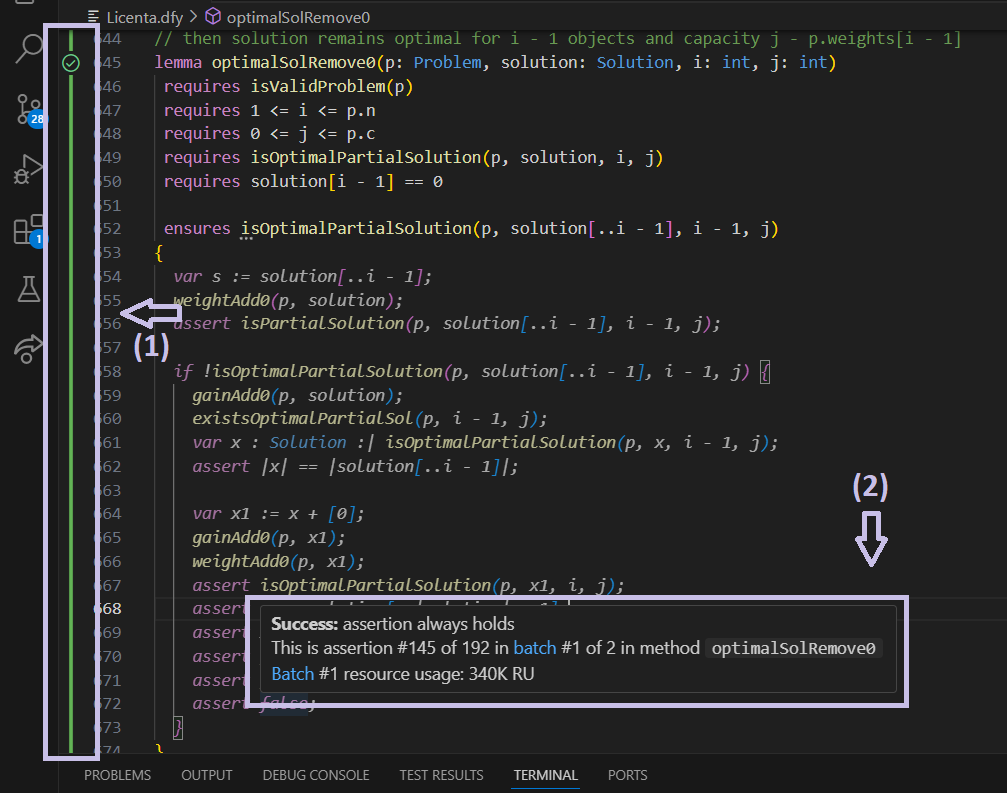
\includegraphics[width=1.0\linewidth]{images/imageVerificationSucceeded.png}
\end{figure}
 \par De exemplu, pentru lema \formatText{optimalSolRemove0} Dafny a reușit să verifice cu succes corectitudinea acesteia, iar acest lucru este evidențiat printr-o bară verticală de culoare verde pe toată lungimea declarației acesteia. În funcție de starea procesului de verificare, această bară își va schimba stilul în mod dinamic pentru a ajuta programatorul în procesul de dezvoltare al codului.
 \par De asemenea, dacă plasăm cursorul peste o instrucțiune, o fereastră pop-up apare în care putem afla informații despre stadiul verificării acesteia (săgeata 2). Acest lucru este de ajutor mai mult în cazul invarianților pentru a afla dacă verificatorul nu poate demonstra corectitudinea acestuia înainte de execuția buclei sau în timpul acesteia. \\ \\ \par
 Pentru a rula algoritmul, avem două variante:
 \begin{itemize}
     \item click dreapta în fișierul ce se dorește a fi rulat și alegem \texttt{Dafny} $\rightarrow$ \texttt{Dafny:Run} (sau \texttt{F5})
     \item din linia de comandă se poate executa următoarea comanda: \texttt{dafny run Licenta.dfy} (mai multe opțiuni de control al verificării pot fi adăugate, precum \texttt{--allow-warnings})
 \end{itemize}
 \par
Una dintre cele mai comune provocări pe care le-am întâmpinat pe parcursul procesului de implementare a fost depășirea timpului de răspuns alocat pentru verificarea unei leme sau a unei metode, care poate apărea atunci când unele specificații nu sunt complete sau când logica demonstrației este mult prea complexă pentru verificator, dar există și cazuri în care acesta se pierde încercând să demonstreze lanțuri inutile de raționament. În astfel de cazuri am avut la îndemană următoarele posibilități:
\begin{itemize}
    \item Utilizarea instrucțiunilor \formatText{assert}: acestea sunt folosite pentru a verifica valoarea de adevăr a unei expresii logice necesare în demonstrație. Cu ajutorul acestora am verificat dacă Dafny poate aproba raționamentul pe care l-am aplicat în demonstrarea postcondițiilor deoarece de foarte multe ori a fost nevoie să ghidez verificatorul spre o anumită direcție logică, dar și unele proprietăți care trebuiau să fie adevărate după apelarea unor leme pentru a continua verificarea. Un exemplu foarte bun pentru ambele cazuri este lema \formatText{gainAddTooBig}:
   \begin{Verbatim}[commandchars=\\\{\}]
\PY{k+kd}{lemma} \PY{n+nf}{gainAddTooBig}\PY{p}{(}\PY{n}{p}\PY{p}{:} \PY{n}{Problem}\PY{p}{,} \PY{n}{solution}\PY{p}{:} \PY{n}{Solution}\PY{p}{,} 
    \PY{n}{i}\PY{p}{:} \PY{k+kt}{int}\PY{p}{,} \PY{n}{j}\PY{p}{:} \PY{k+kt}{int}\PY{p}{)} 
 \PY{p}{..}\PY{p}{.}
 \PY{k}{requires} \PY{n}{isPartialSolution}\PY{p}{(}\PY{n}{p}\PY{p}{,} \PY{n}{solution}\PY{p}{,} \PY{n}{i}\PY{p}{,} \PY{n}{j}\PY{p}{)}
 \PY{k}{requires} \PY{n}{p}\PY{p}{.}\PY{n}{weights}\PY{p}{[}\PY{n}{i} \PY{o}{\PYZhy{}} \PY{l+m+mi}{1}\PY{p}{]} \PY{o}{\PYZgt{}} \PY{n}{j}
 \PY{k}{ensures} \PY{n}{solution}\PY{p}{[}\PY{n}{i} \PY{o}{\PYZhy{}} \PY{l+m+mi}{1}\PY{p}{]} \PY{o}{==} \PY{l+m+mi}{0}
 \PY{k}{ensures} \PY{n}{gain}\PY{p}{(}\PY{n}{p}\PY{p}{,} \PY{n}{solution}\PY{p}{[}\PY{p}{..}\PY{n}{i} \PY{o}{\PYZhy{}} \PY{l+m+mi}{1}\PY{p}{]}\PY{p}{)} \PY{o}{==} \PY{n}{gain}\PY{p}{(}\PY{n}{p}\PY{p}{,} \PY{n}{solution}\PY{p}{)}
 \PY{p}{\PYZob{}}
    \PY{k}{if} \PY{n}{solution}\PY{p}{[}\PY{n}{i} \PY{o}{\PYZhy{}} \PY{l+m+mi}{1}\PY{p}{]} \PY{o}{==} \PY{l+m+mi}{1} \PY{p}{\PYZob{}}
      \PY{k}{assert} \PY{n}{computeWeight}\PY{p}{(}\PY{n}{p}\PY{p}{,} \PY{n}{solution}\PY{p}{,} \PY{o}{|}\PY{n}{solution}\PY{o}{|} \PY{o}{\PYZhy{}} \PY{l+m+mi}{1}\PY{p}{)} \PY{o}{==} 
        \PY{n}{computeWeight}\PY{p}{(}\PY{n}{p}\PY{p}{,} \PY{n}{solution}\PY{p}{,} \PY{o}{|}\PY{n}{solution}\PY{p}{[}\PY{p}{..}\PY{n}{i}\PY{p}{]}\PY{o}{|} \PY{o}{\PYZhy{}} \PY{l+m+mi}{1}\PY{p}{)} \PY{o}{+} 
        \PY{n}{p}\PY{p}{.}\PY{n}{weights}\PY{p}{[}\PY{n}{i} \PY{o}{\PYZhy{}} \PY{l+m+mi}{1}\PY{p}{]}\PY{p}{;}
      \PY{k}{assert} \PY{n}{weight}\PY{p}{(}\PY{n}{p}\PY{p}{,} \PY{n}{solution}\PY{p}{)} \PY{o}{\PYZgt{}=} \PY{n}{p}\PY{p}{.}\PY{n}{weights}\PY{p}{[}\PY{n}{i} \PY{o}{\PYZhy{}} \PY{l+m+mi}{1}\PY{p}{]} \PY{o}{\PYZgt{}} \PY{n}{j}\PY{p}{;}
      \PY{k}{assert} \PY{err}{!}\PY{n}{isPartialSolution}\PY{p}{(}\PY{n}{p}\PY{p}{,} \PY{n}{solution}\PY{p}{,} \PY{n}{i}\PY{p}{,} \PY{n}{j}\PY{p}{)}\PY{p}{;}
      \PY{k}{assert} \PY{k+kc}{false}\PY{p}{;}
    \PY{p}{\PYZcb{}}
    \PY{k}{assert} \PY{n}{solution}\PY{p}{[}\PY{n}{i} \PY{o}{\PYZhy{}} \PY{l+m+mi}{1}\PY{p}{]} \PY{o}{==} \PY{l+m+mi}{0}\PY{p}{;}
    \PY{n}{computeGainAdd0}\PY{p}{(}\PY{n}{p}\PY{p}{,} \PY{n}{solution}\PY{p}{,} \PY{o}{|}\PY{n}{solution}\PY{o}{|} \PY{o}{\PYZhy{}} \PY{l+m+mi}{2}\PY{p}{)}\PY{p}{;}
    \PY{k}{assert} \PY{n}{gain}\PY{p}{(}\PY{n}{p}\PY{p}{,} \PY{n}{solution}\PY{p}{[}\PY{p}{..}\PY{n}{i} \PY{o}{\PYZhy{}} \PY{l+m+mi}{1}\PY{p}{]}\PY{p}{)} \PY{o}{==} \PY{n}{gain}\PY{p}{(}\PY{n}{p}\PY{p}{,} \PY{n}{solution}\PY{p}{)}\PY{p}{;}
\PY{p}{\PYZcb{}}
\end{Verbatim}
    unde assert-urile din instrucțiunea $if$ urmăresc să ajungem la o contradicție prin faptul că soluția nu are cum să fie parțială dacă greutatea obiectului depășește capacitatea $j$, propoziție care este falsă deoarece avem o precondiție care asigură exact acest lucru, iar instrucțiunea 
    \begin{Verbatim}[commandchars=\\\{\}]
\PY{k}{assert} \PY{n}{gain}\PY{p}{(}\PY{n}{p}\PY{p}{,} \PY{n}{solution}\PY{p}{[}\PY{p}{..}\PY{n}{i} \PY{o}{\PYZhy{}} \PY{l+m+mi}{1}\PY{p}{]}\PY{p}{)} \PY{o}{==} \PY{n}{gain}\PY{p}{(}\PY{n}{p}\PY{p}{,} \PY{n}{solution}\PY{p}{)}\PY{p}{;}
\end{Verbatim}
    se asigură că după apelarea lemei computeGainAdd0 verificatorul știe că profitul unei soluții rămâne neschimbat dacă eliminăm ultimul element de 0 din soluție. \par
    \hspace{2mm} De asemenea, folosind structura \texttt{assert ... by} putem reduce sarcina verificatorului deoarece pașii din acest bloc de instrucțiuni sunt uitați după verificarea condiției din assert:
    \begin{Verbatim}[commandchars=\\\{\}]
\PY{k}{assert} \PY{n}{gain}\PY{p}{(}\PY{n}{p}\PY{p}{,} \PY{n}{x}\PY{p}{[}\PY{p}{..}\PY{n}{i} \PY{o}{\PYZhy{}} \PY{l+m+mi}{1}\PY{p}{]}\PY{p}{)} \PY{o}{==} \PY{n}{gain}\PY{p}{(}\PY{n}{p}\PY{p}{,} \PY{n}{solution1}\PY{p}{)} \PY{n}{by}
\PY{p}{\PYZob{}}
  \PY{n}{optimalSolRemove1}\PY{p}{(}\PY{n}{p}\PY{p}{,} \PY{n}{x}\PY{p}{,} \PY{n}{i}\PY{p}{,} \PY{n}{j}\PY{p}{)}\PY{p}{;}
  \PY{k}{assert} \PY{n}{isOptimalPartialSolution}\PY{p}{(}\PY{n}{p}\PY{p}{,} \PY{n}{x}\PY{p}{[}\PY{p}{..}\PY{n}{i} \PY{o}{\PYZhy{}} \PY{l+m+mi}{1}\PY{p}{]}\PY{p}{,} 
    \PY{n}{i} \PY{o}{\PYZhy{}} \PY{l+m+mi}{1}\PY{p}{,} \PY{n}{j} \PY{o}{\PYZhy{}} \PY{n}{p}\PY{p}{.}\PY{n}{weights}\PY{p}{[}\PY{n}{i} \PY{o}{\PYZhy{}} \PY{l+m+mi}{1}\PY{p}{]}\PY{p}{)}\PY{p}{;}
\PY{p}{\PYZcb{}} 
\end{Verbatim}
    \item Utilizarea instrucțiunii \formatText{assume}: această instrucțiune este foarte utilă pentru a determina la ce linie întâlnește Dafny probleme. O instrucțiune assume tratează condiția ca fiind adevarată, de aceea de multe ori am folosit-o pentru a afla de ce informații în plus are nevoie verificatorul sau pentru a putea continua următorii pași ai demonstrației. De exemplu, mi-a fost de ajutor în cazul lemelor în care presupun că există o lemă mai bună decât cea pentru care vreau să demonstrez că este optimă, întrucât am putut continua implementarea acestora, după care am revenit să formulez o lemă specială pentru existența unor astfel de soluții. \par
    \hspace{2mm} O altă utilizare a instrucțiunii assume a fost \texttt{assume false;} care oprește verificarea pentru condițiile ce urmează după aceasta și îi indică verificatorului să nu mai încerce demonstrarea acestora și să accepte orice afirmație ulterioară ca fiind adevărată. Aceasta instrucțiune a fost foarte folositoare pentru a identifica ce assert-uri nu reușea Dafny să demonstreze pentru lemele mai complexe, mai ales în cazul instrucțiunilor $if$ din cadrul lemelor unde pe fiecare ramură aveam o logică diferită și ambele puteau cauza probleme de logică.
    \item \formatText{Refactorizarea codului}: în leme precum \formatText{optimalSolAdd1} sau \formatText{optimalSolAdd0}, unde deși demonstrația era corectă și fiecare caz (când ultimul element este fie 0, fie 1) se verifica cu succes separat, dacă ambele erau tratate în cadrul aceleași leme obțineam acest timeout deoarece demonstrația era destul de complexă pentru Dafny. Soluția a fost astfel să tratez unul dintre cele două cazuri posibile într-o lemă separată.
\end{itemize}
\end{sloppypar}